\subsection{part b}
Now design PID controller with following methods.
\newpage
\begin{itemize}
    \item ziegler nichols
    $$
    G_c =   \dfrac{4.756 s^2 + 6.423 s + 2.27}{0.1904 s^2 + 2.76 s}
    $$
    \begin{figure}[H]
        \caption{step responde with ziegler nichols PID controller}
        \centering
        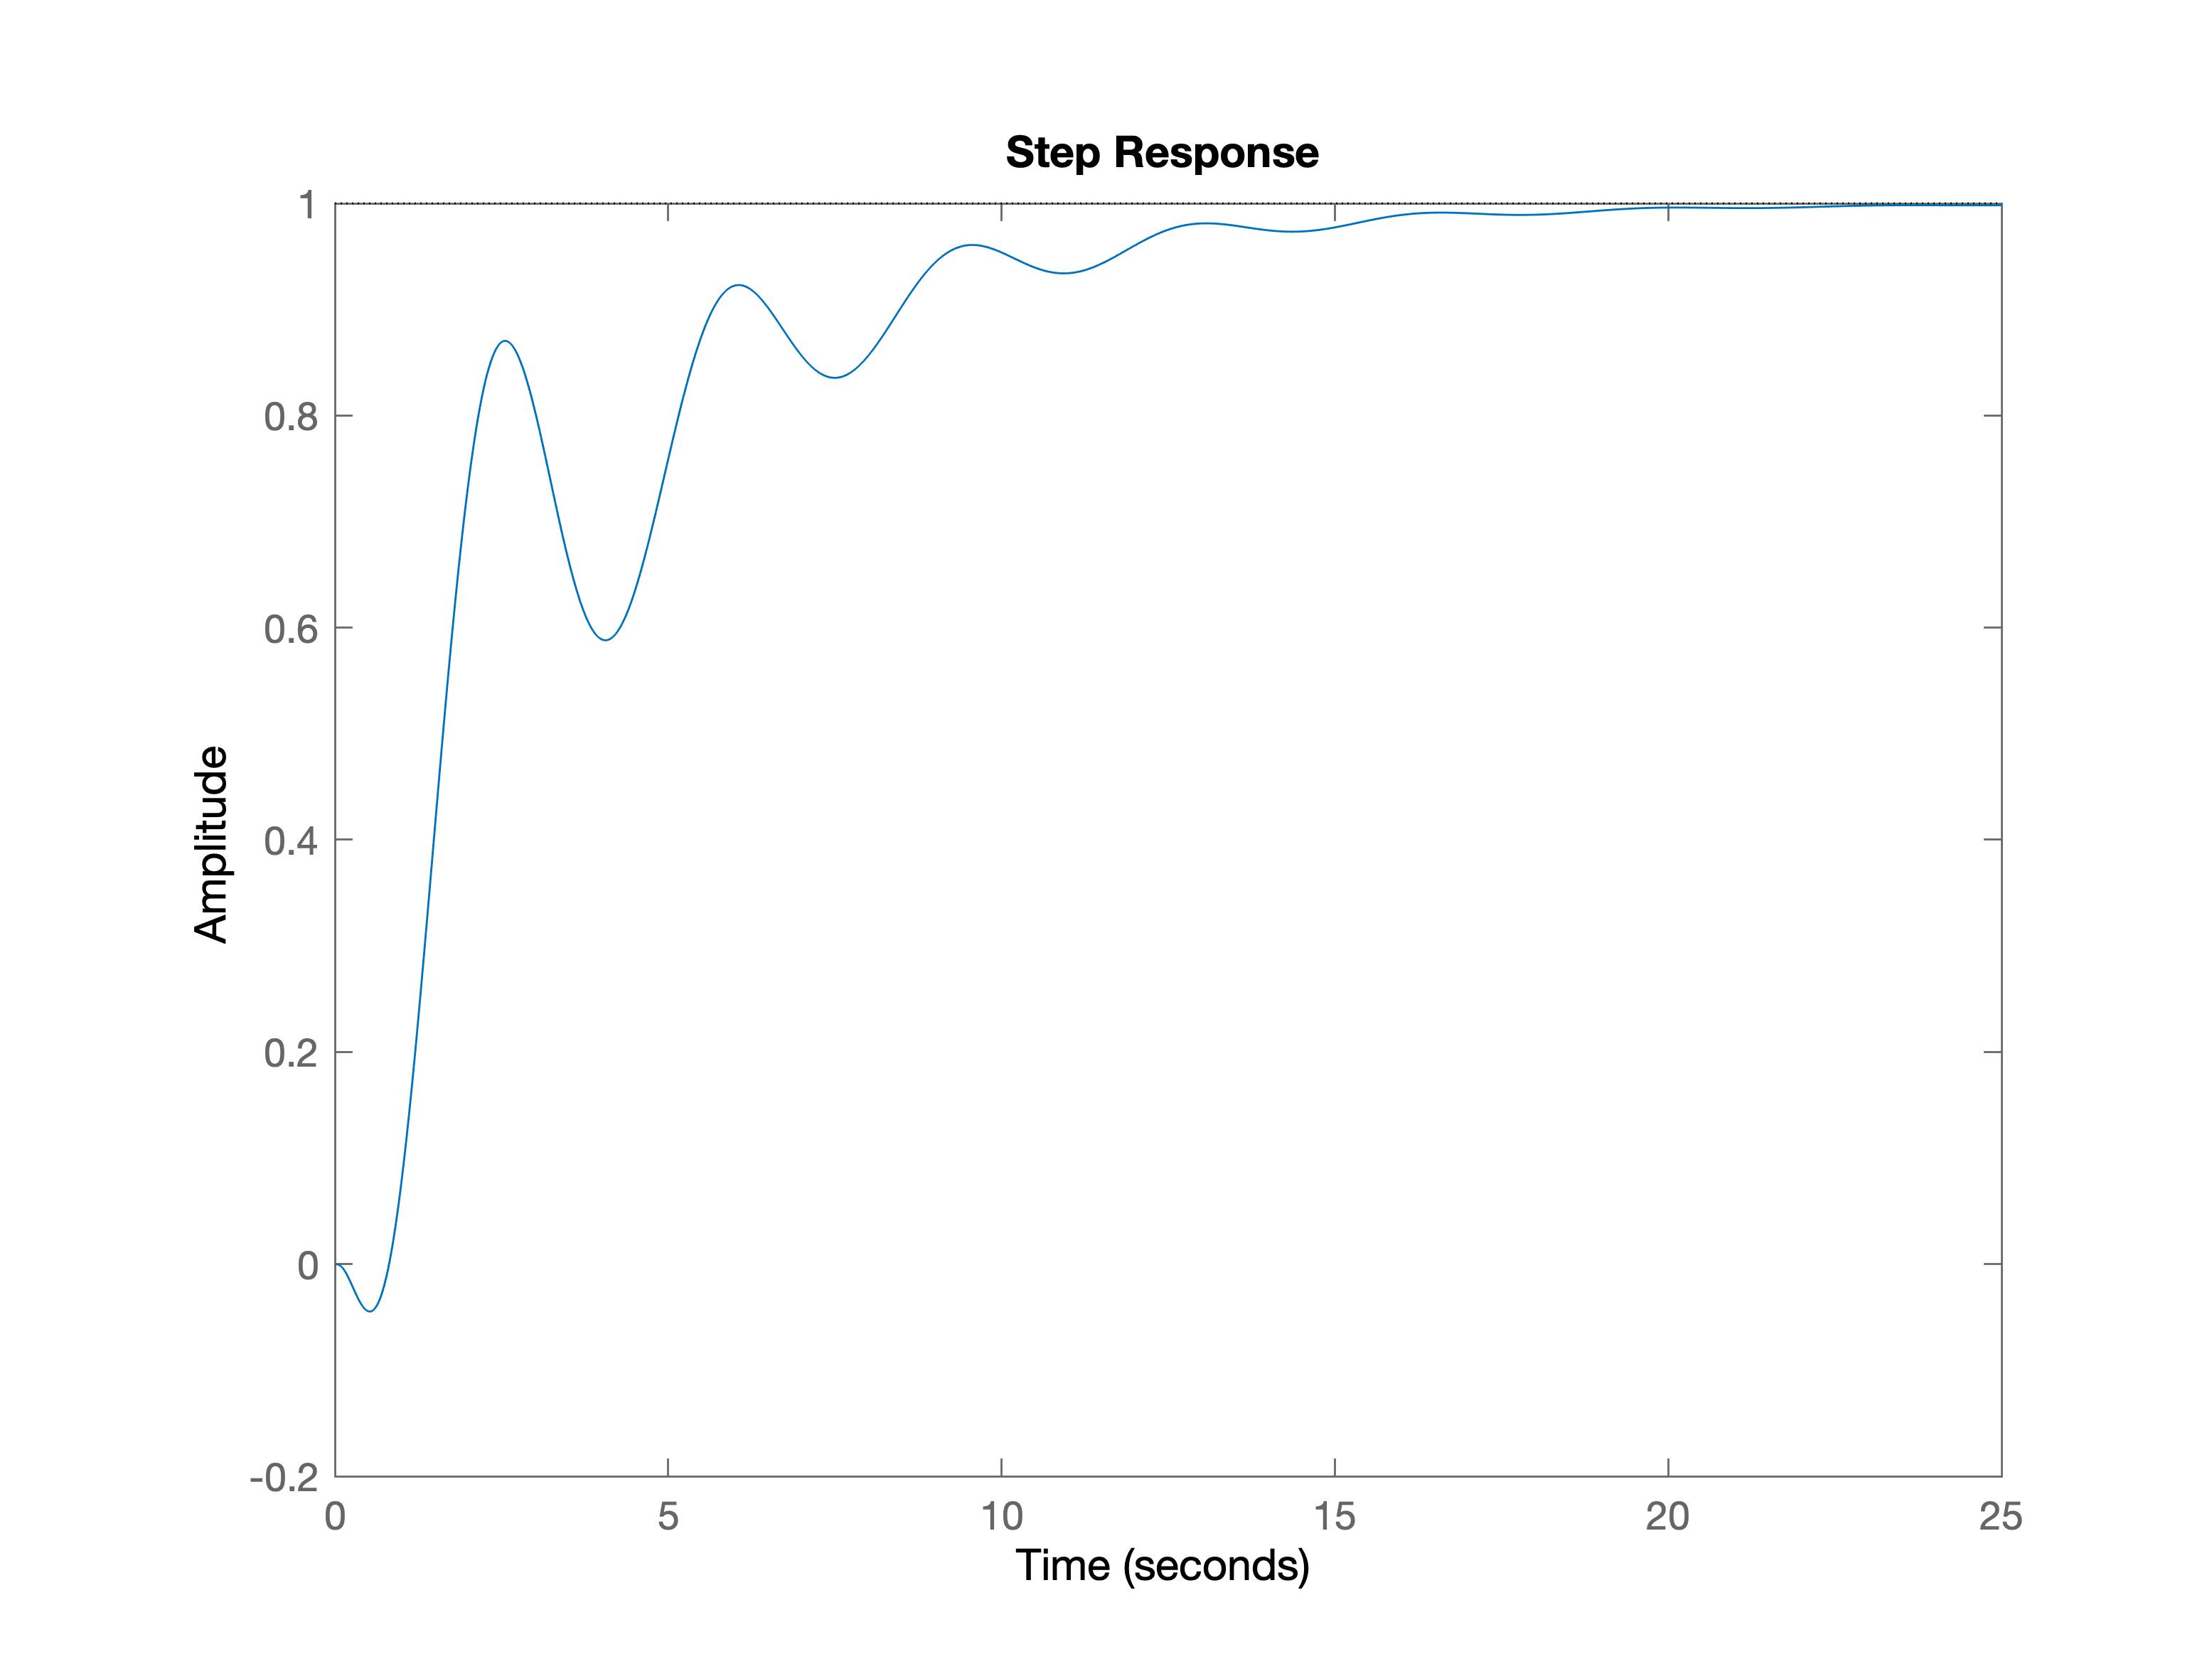
\includegraphics[width=10cm]{../Figure/Q1/b/zn.png}
    \end{figure}
    \item refined ziegler nichols
    $$
    G_c =     \dfrac{3.099 s + 2.27}{1.629 s}, \qquad H =    
    \dfrac{1.051 s^2 + 1.698 s + 1}{0.09418 s^2 + 1.434 s + 1}
    $$
    \begin{figure}[H]
        \caption{step responde with refined ziegler nichols PID controller}
        \centering
        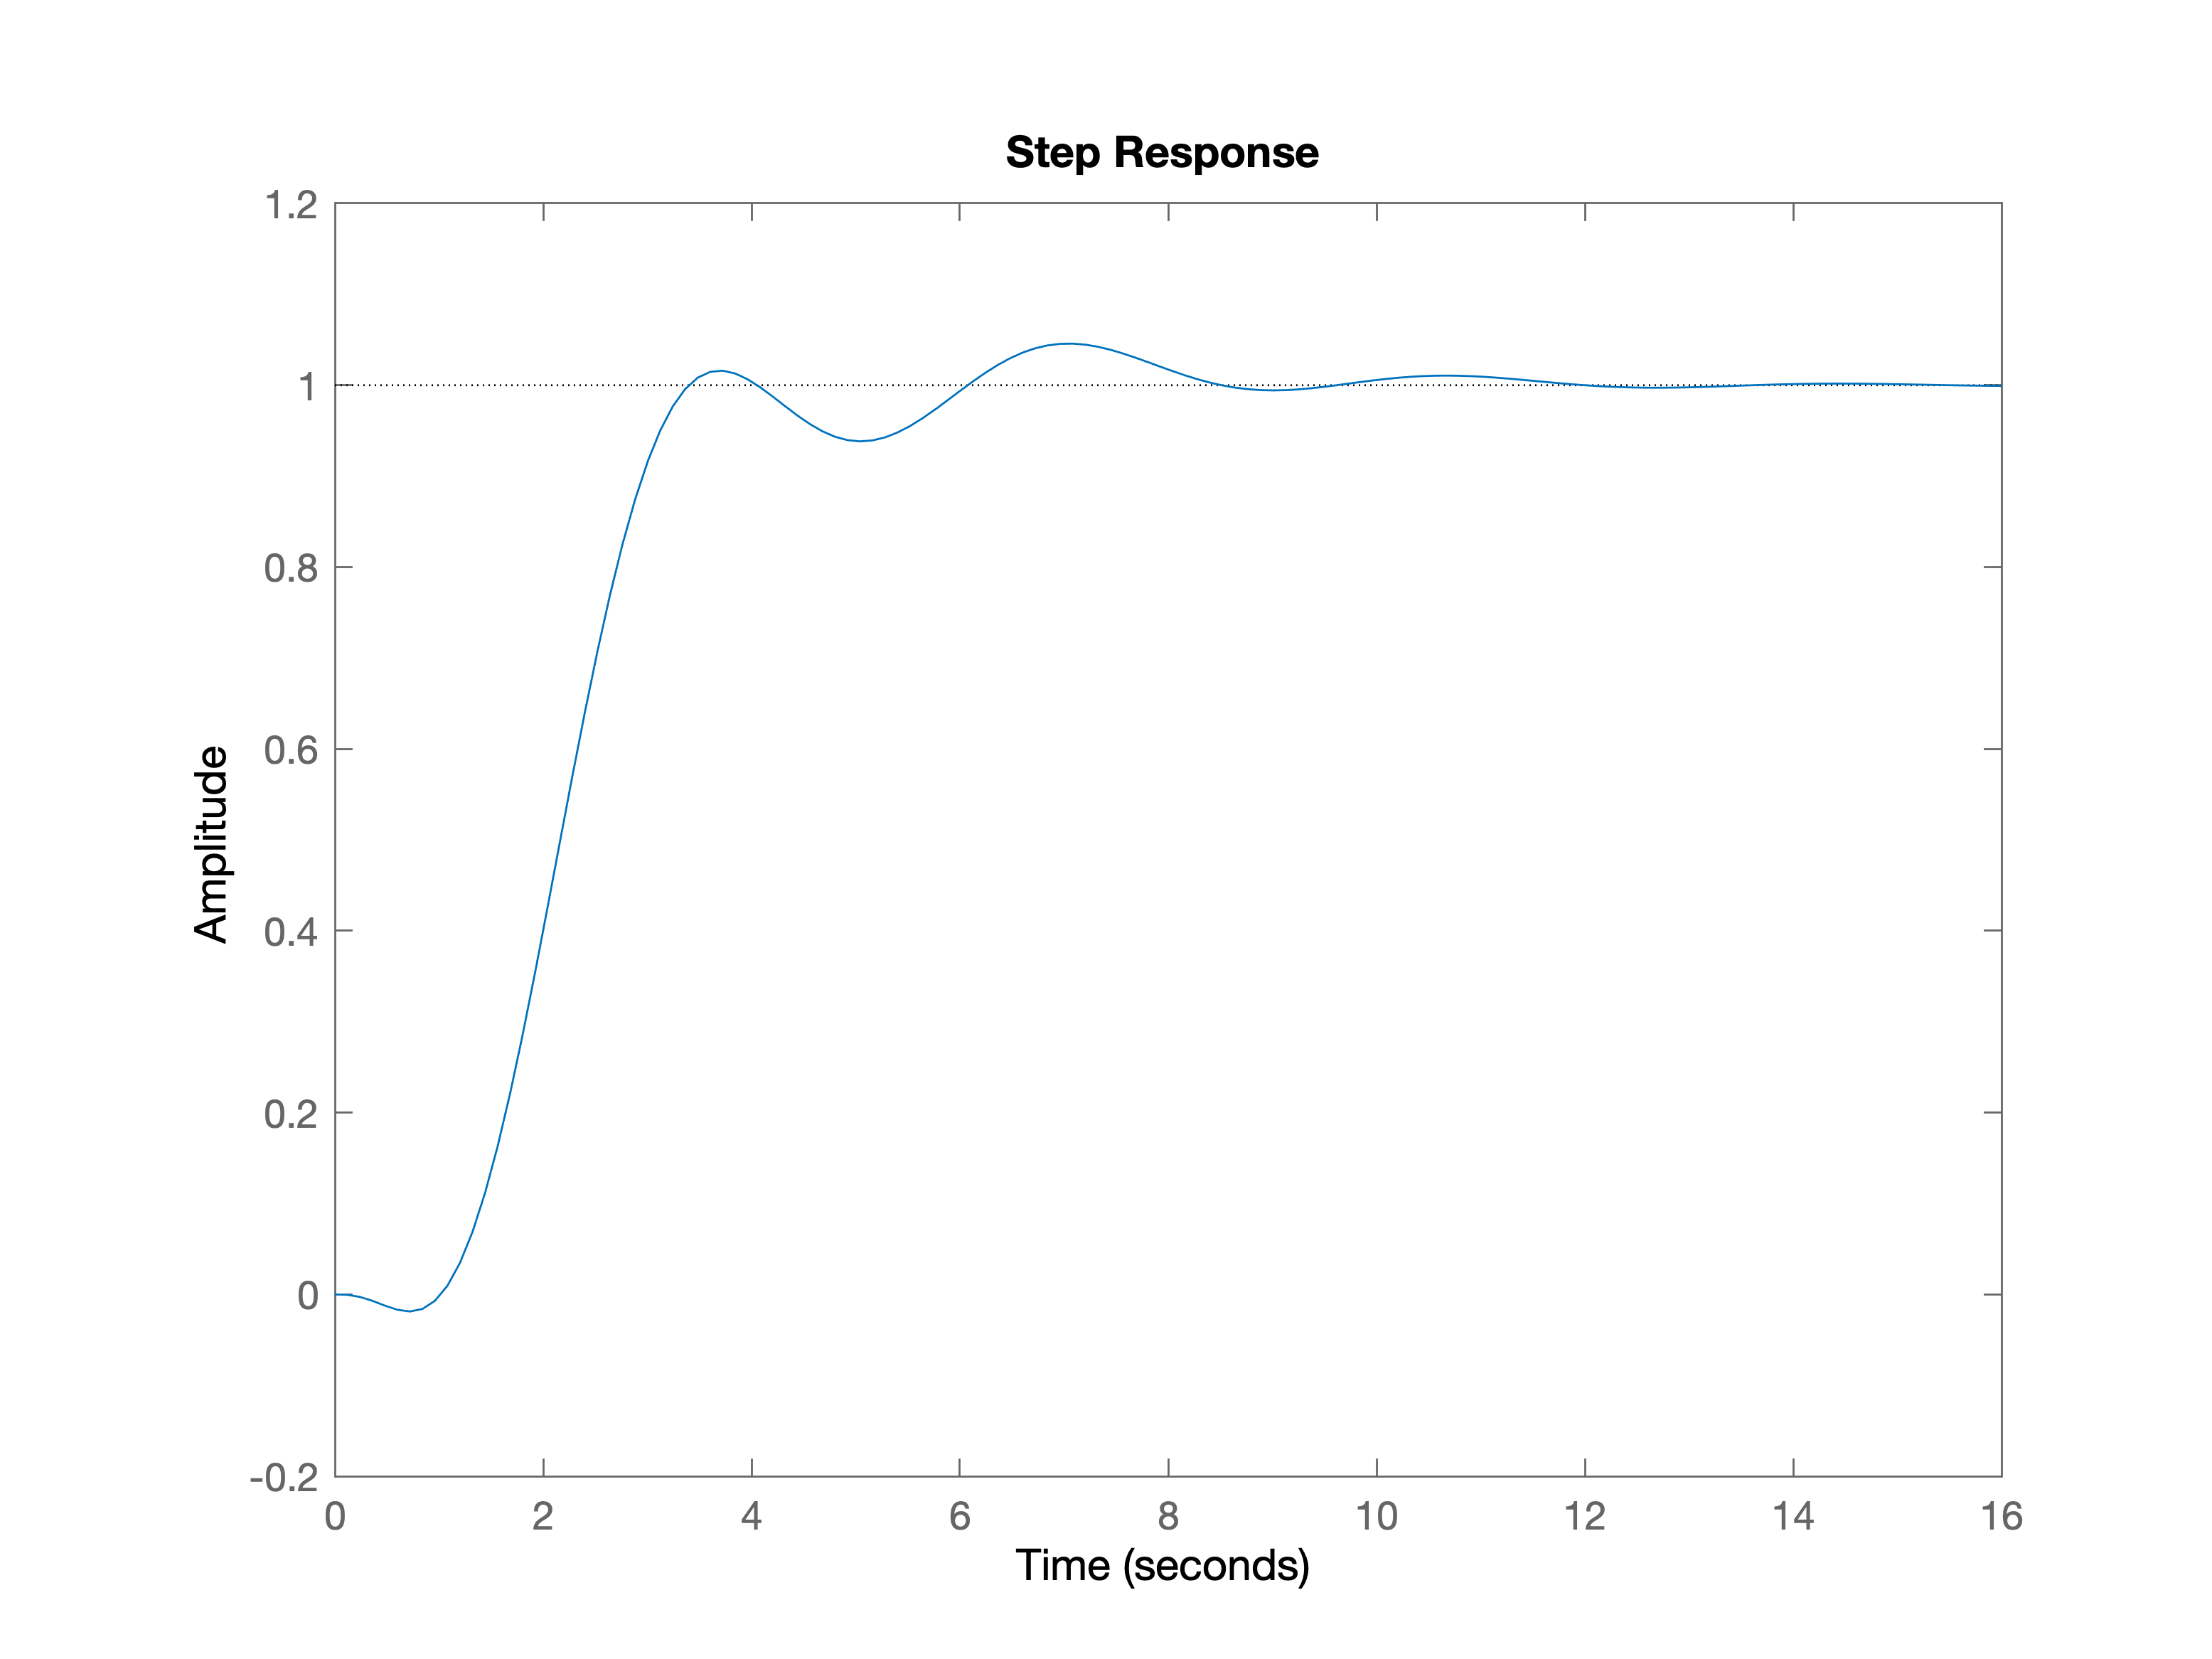
\includegraphics[width=10cm]{../Figure/Q1/b/rzn.png}
    \end{figure}
    \item modified ziegler nichols
    $$
    r_1 = 1.0, \qquad p_b = 5:5:35
    $$
    \begin{figure}[H]
        \caption{step responde with modified ziegler nichols PID controller}
        \centering
        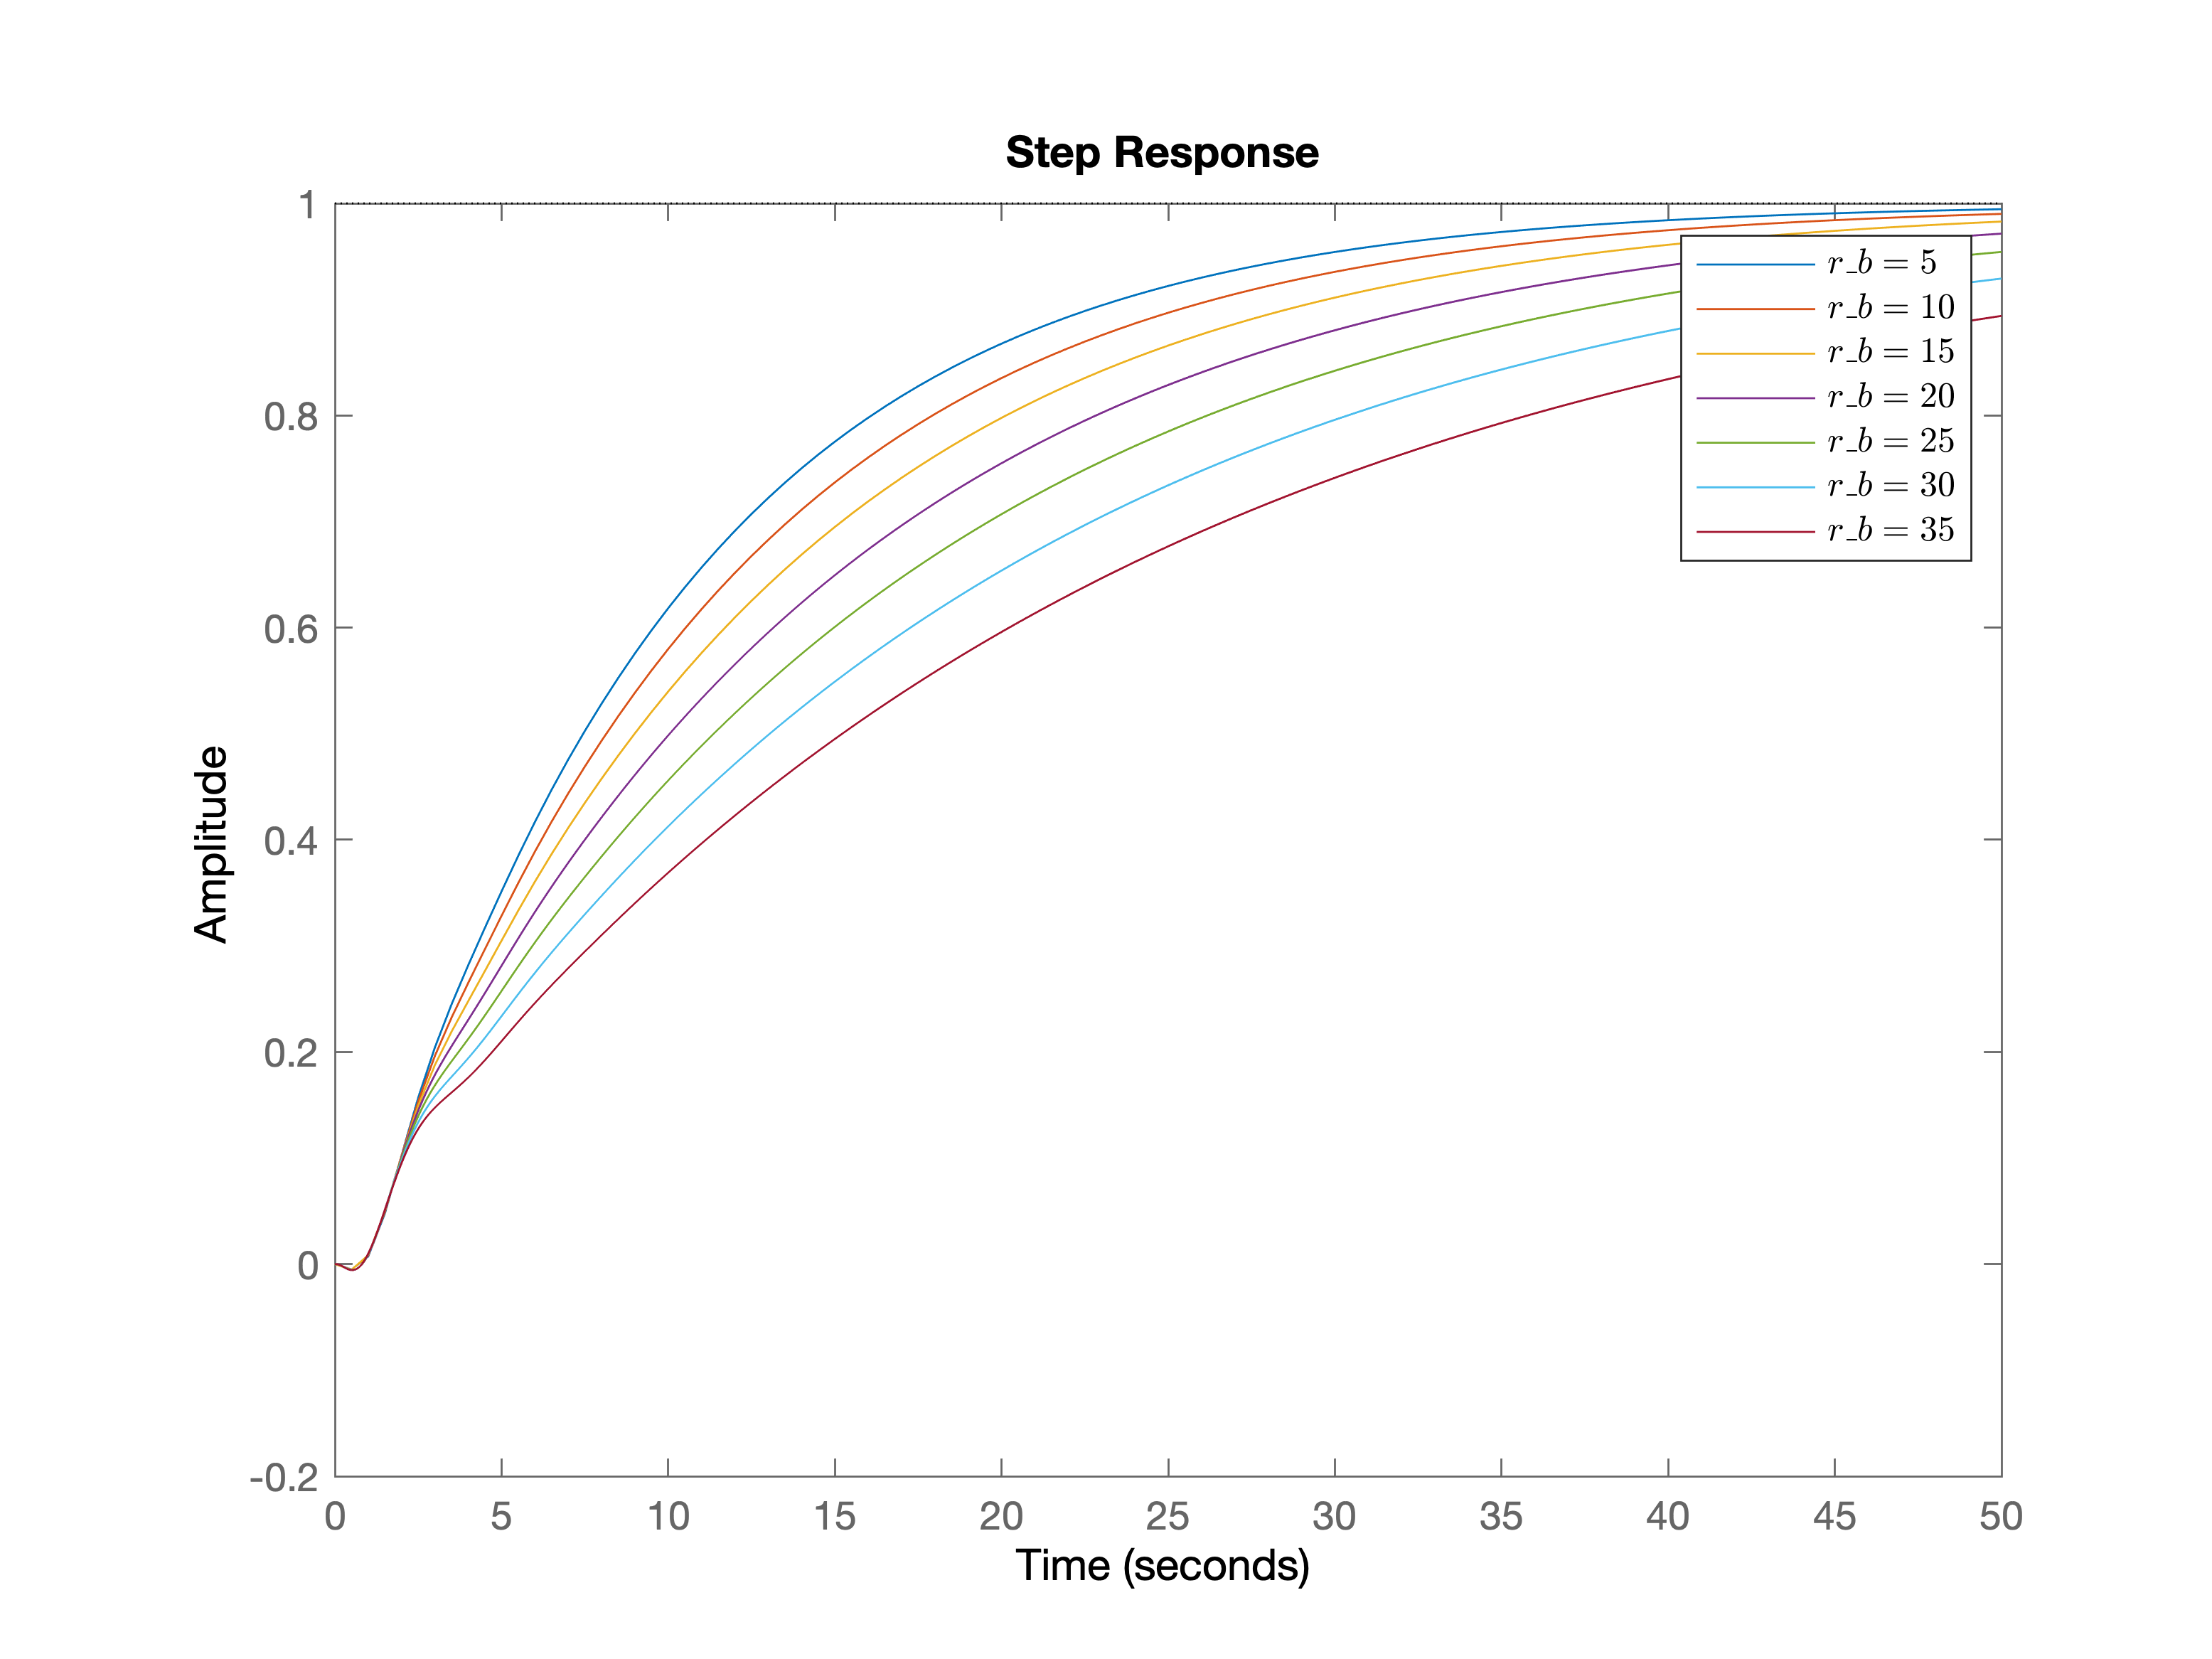
\includegraphics[width=10cm]{../Figure/Q1/b/mzn.png}
    \end{figure}
    \item Cohen Coon
    $$
    G_c =   \dfrac{3.223 s^2 + 7.463 s + 3.189}{ 0.09188 s^2 + 2.3 s}
    $$
    \begin{figure}[H]
        \caption{step responde with Cohen Coon PID controller}
        \centering
        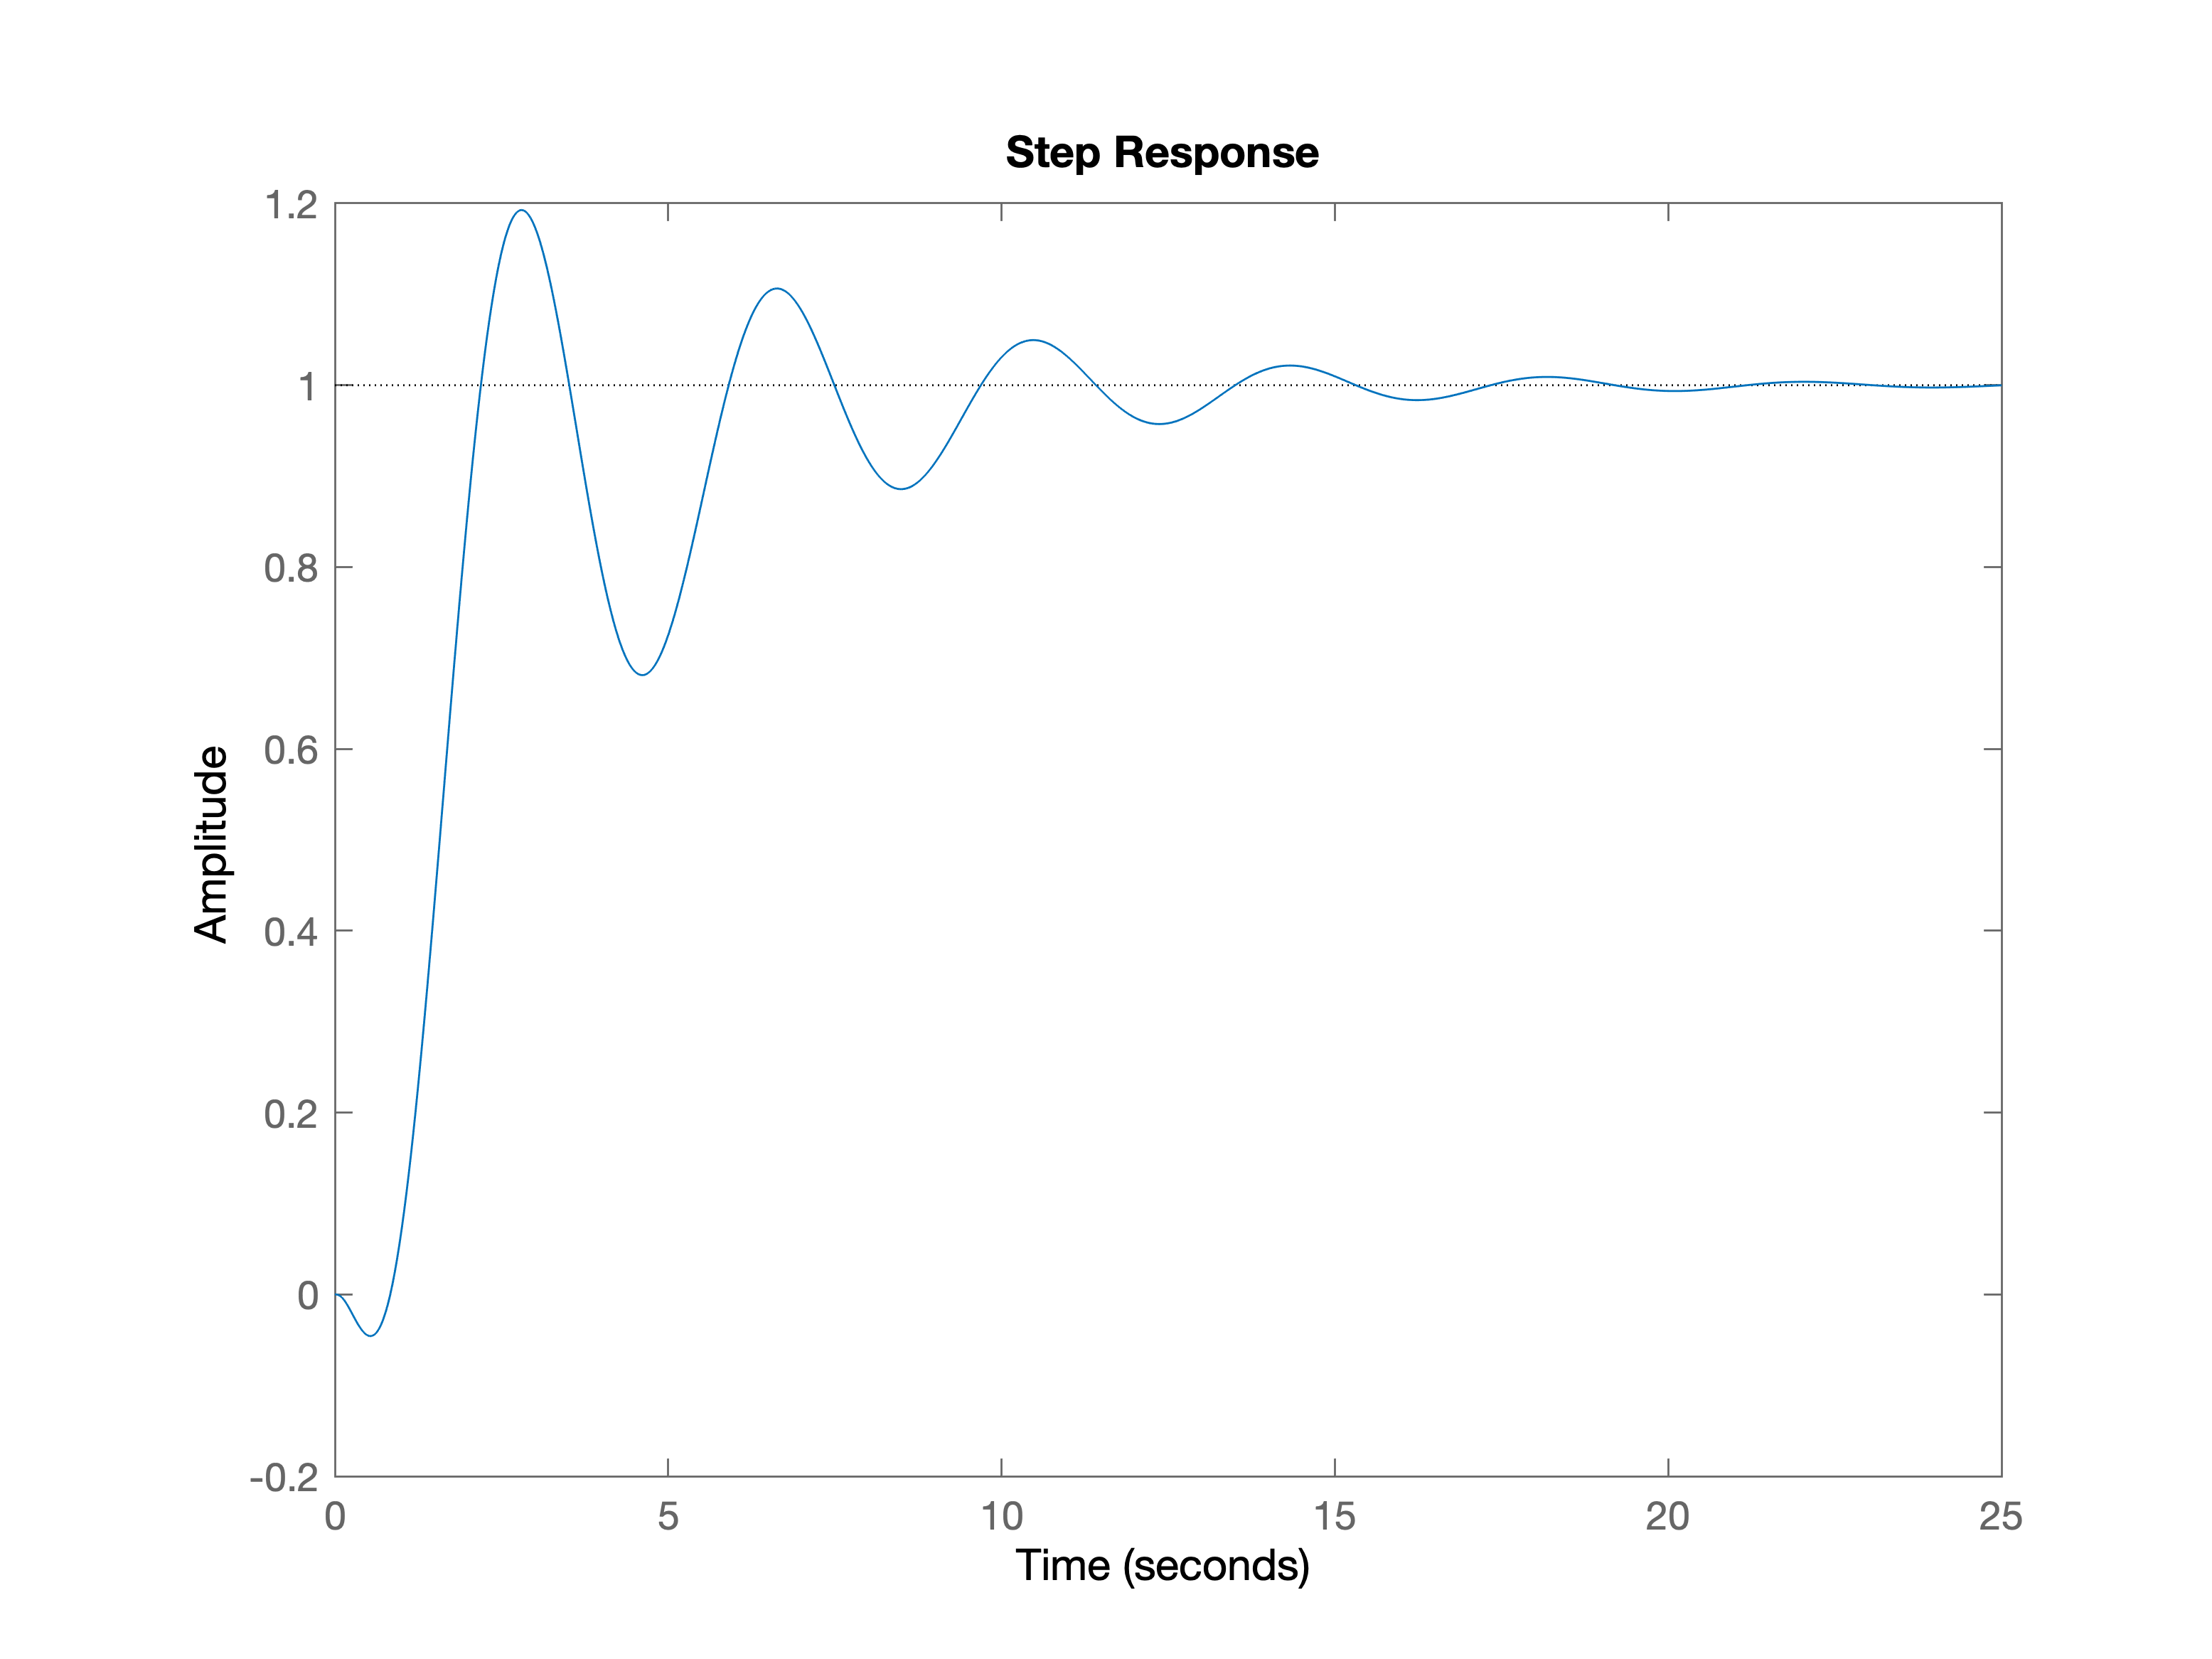
\includegraphics[width=10cm]{../Figure/Q1/b/cc.png}
    \end{figure}
    \newpage
    \item Cohen Coon revisited
    $$
    G_c =   \dfrac{3.374 s^2 + 7.744 s + 3.202}{0.09579 s^2 + 2.378 s}
    $$ 
    \begin{figure}[H]
        \caption{step responde with Cohen Coon revisited PID controller}
        \centering
        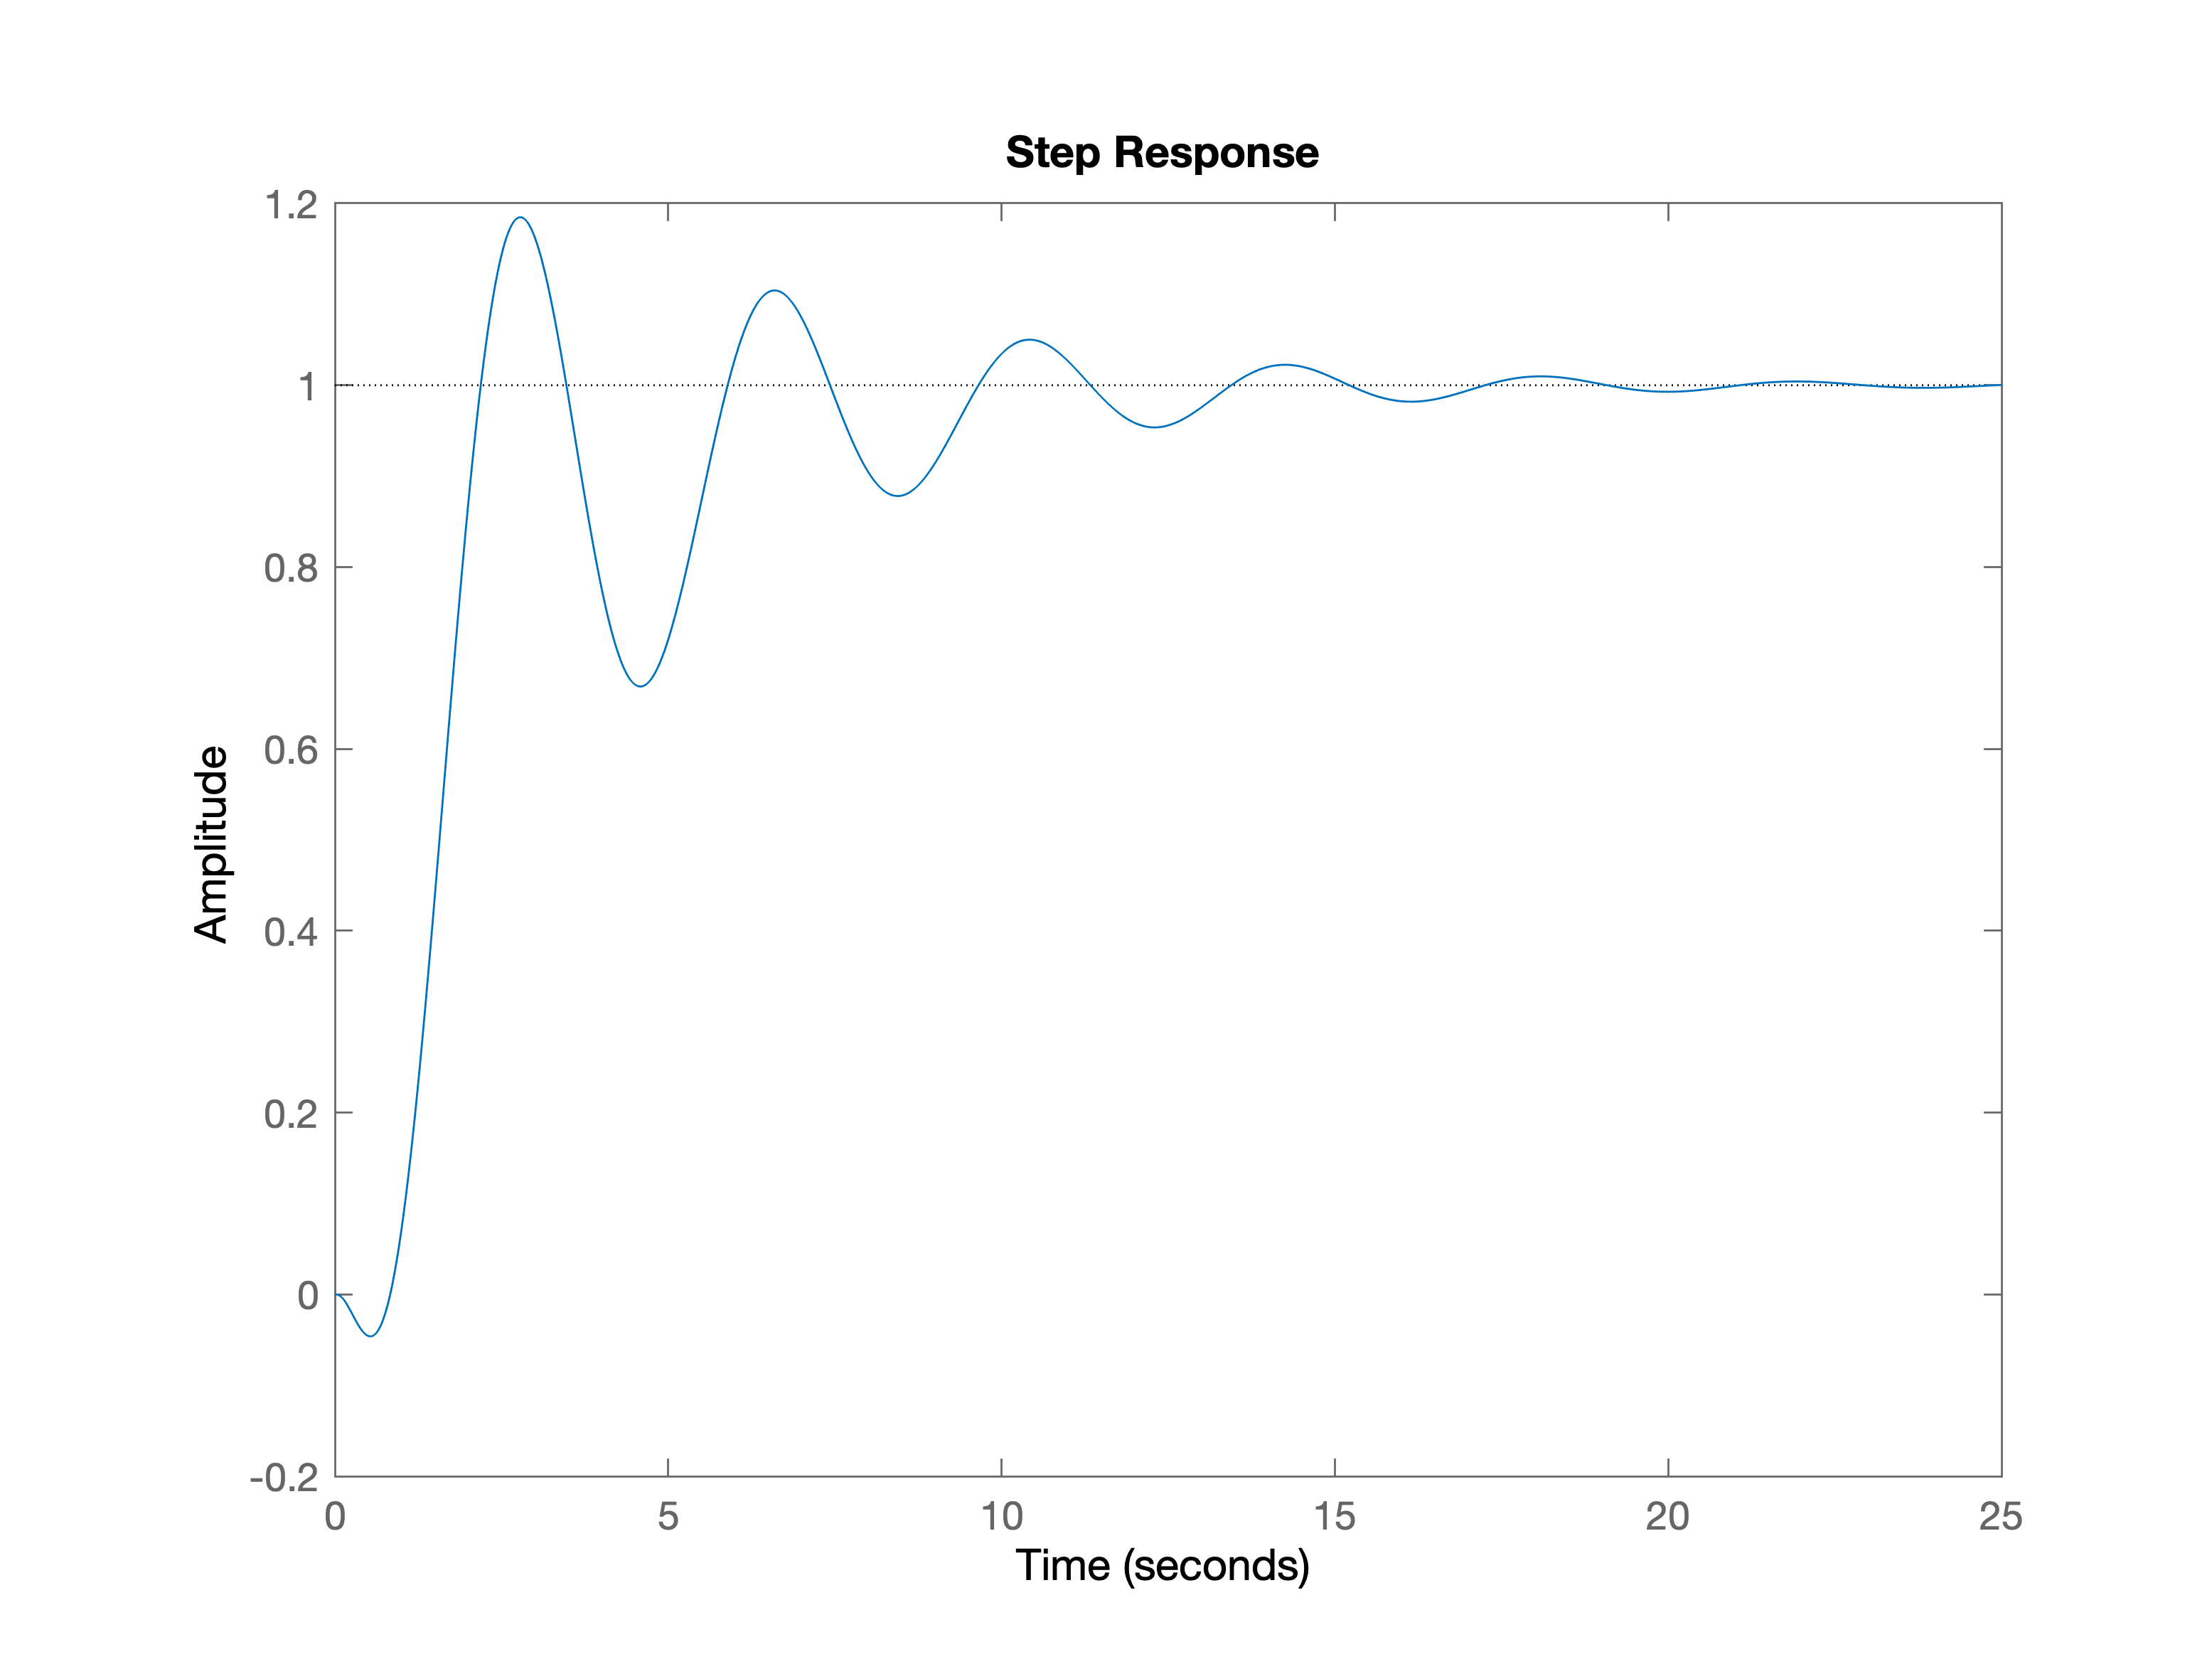
\includegraphics[width=10cm]{../Figure/Q1/b/ccr.png}
    \end{figure} 
    \item Astrom Hagglund
    $$
    G_c =   \dfrac{0.9211 s^2 + 1.794 s + 1.385}{0.06048 s^2 + 1.247 s}
    $$ 
    \begin{figure}[H]
        \caption{step responde with Astrom Hagglund PID controller}
        \centering
        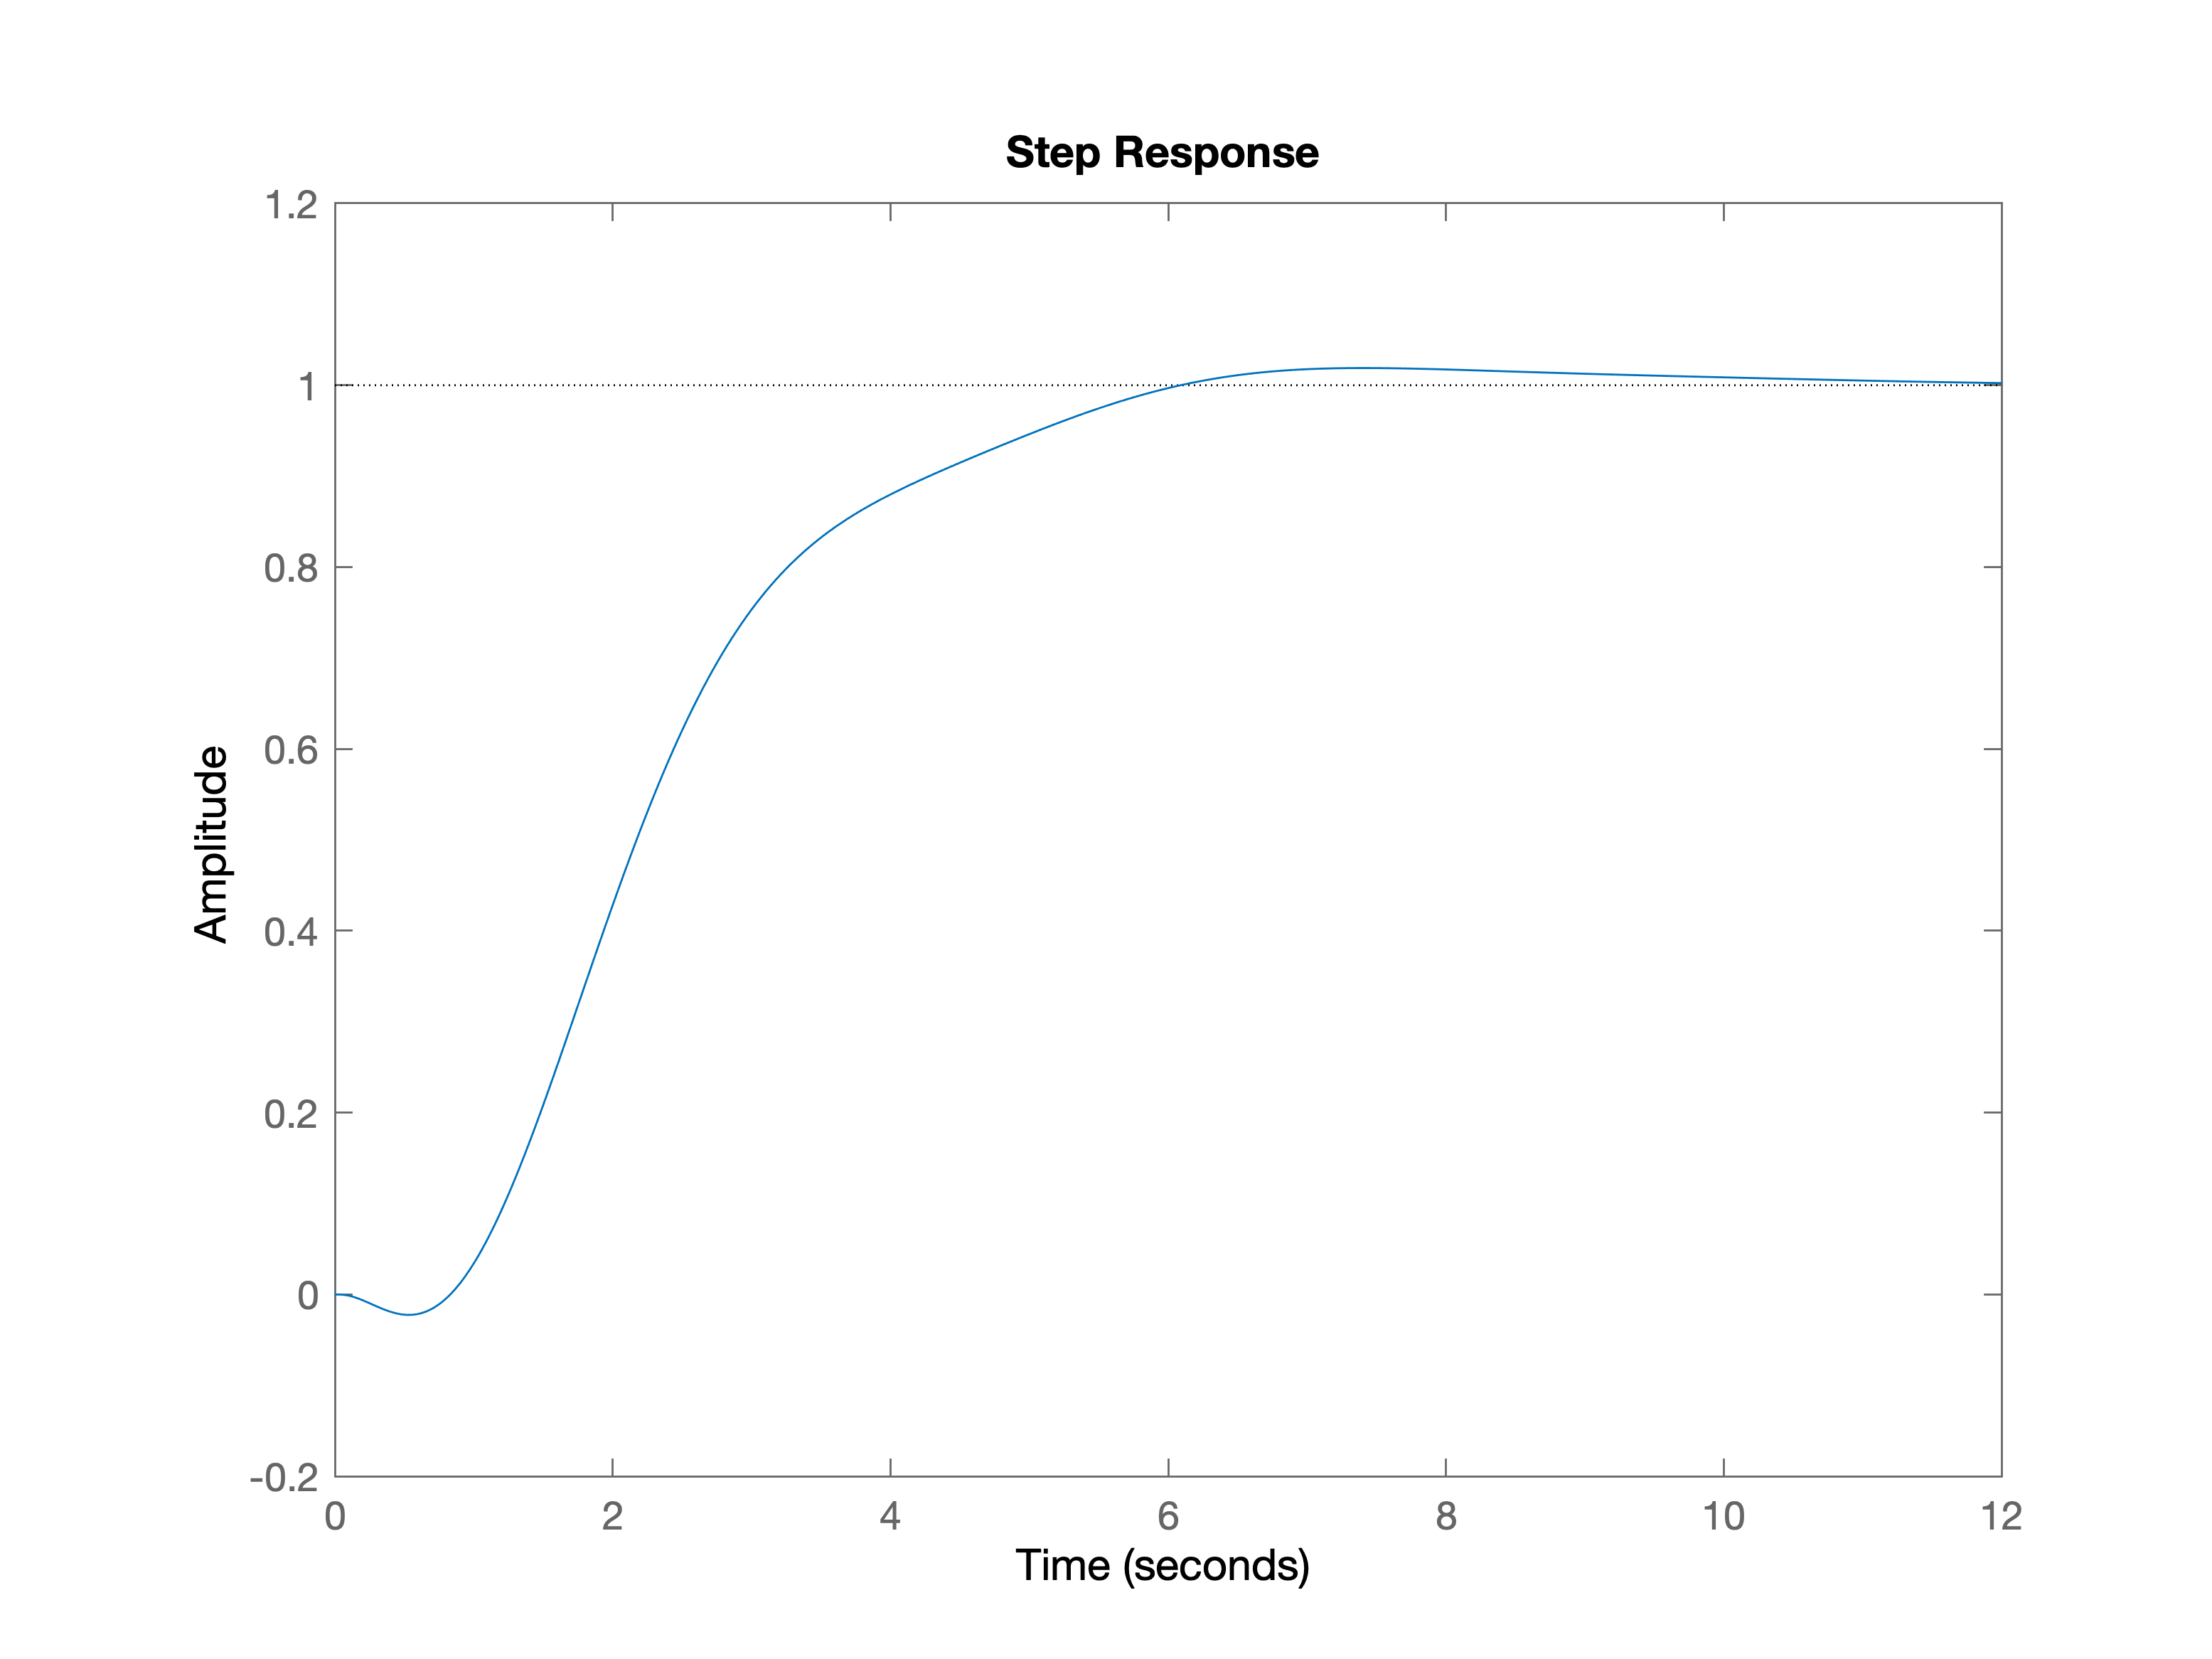
\includegraphics[width=10cm]{../Figure/Q1/b/ah.png}
    \end{figure}  
    \item Frequency based Astrom Hagglund
    $$
    G_c =   \dfrac{1.025 s^2 + 1.666 s + 1.355}{0.0688 s^2 + 1.171 s}
    $$ 
    \begin{figure}[H]
        \caption{step responde with Frequency based Astrom Hagglund PID controller}
        \centering
        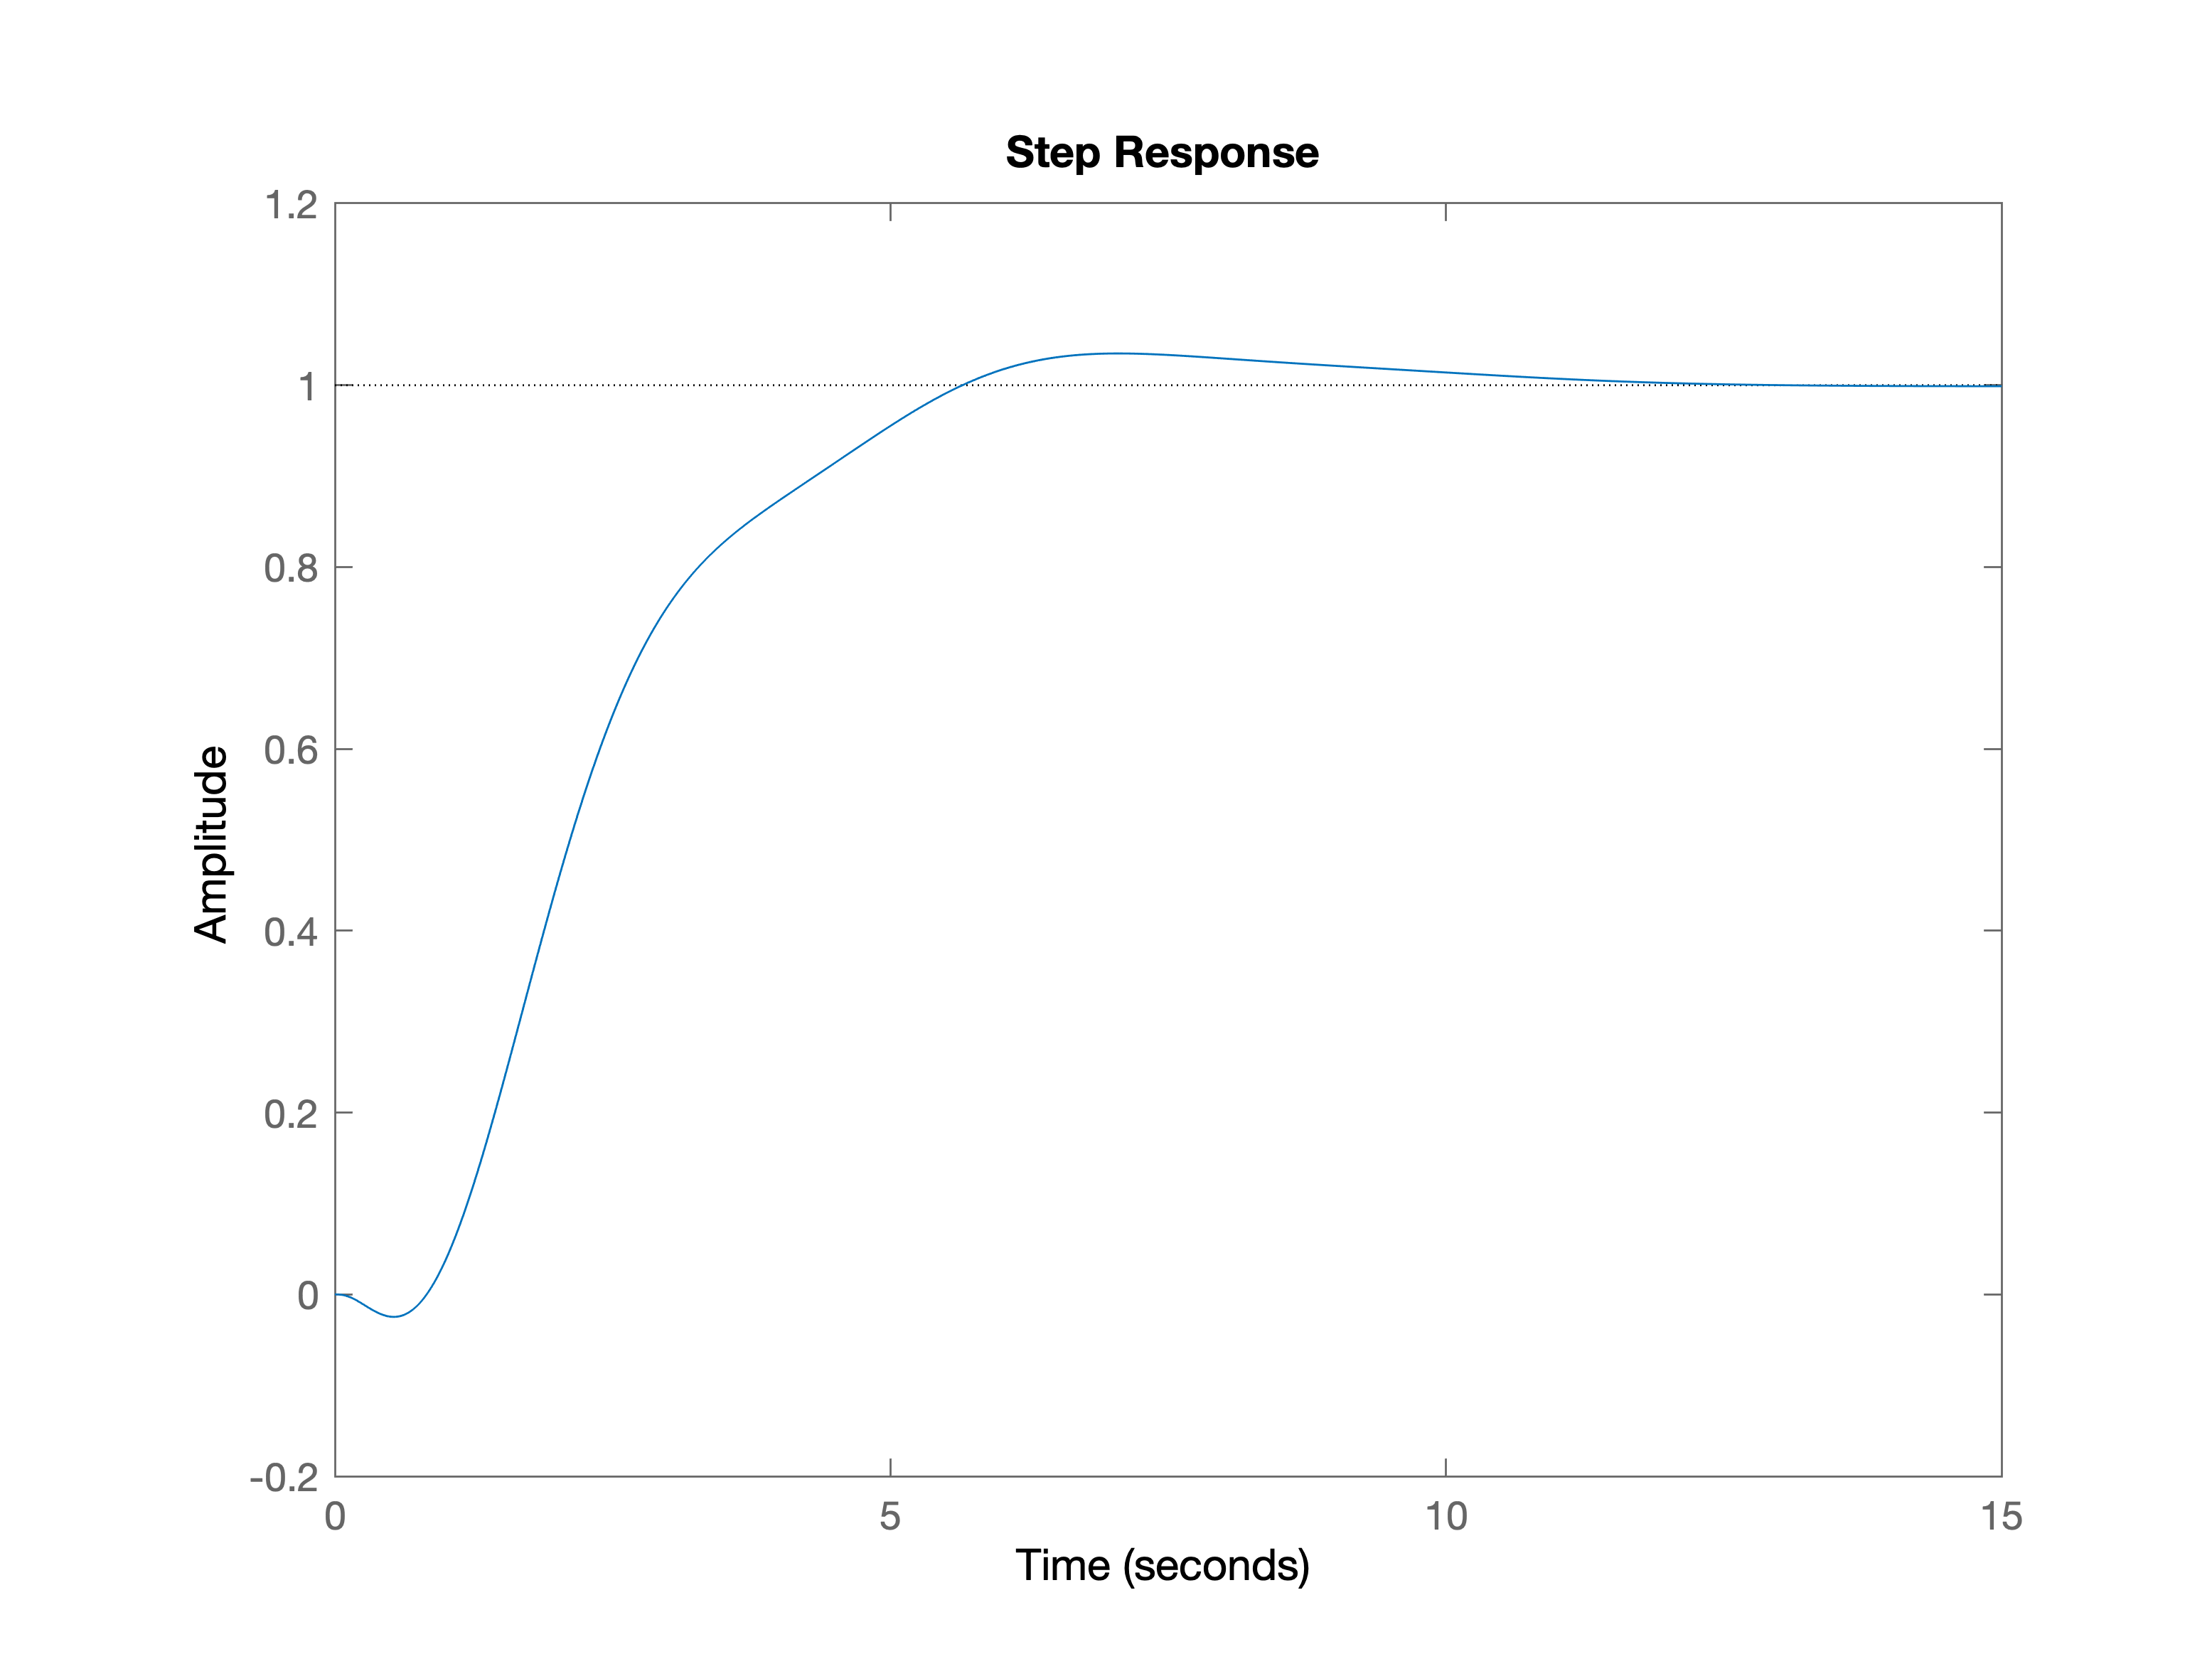
\includegraphics[width=10cm]{../Figure/Q1/b/fah.png}
    \end{figure} 
    \item CHR set point $0\%$ overshoot
    $$
    G_c =   \dfrac{0.8439 s^2 + 1.19 s + 1.135}{0.06758 s^2 + 0.9794 s}
    $$ 
    \begin{figure}[H]
        \caption{step responde with CHR set point $0\%$ overshoot PID controller}
        \centering
        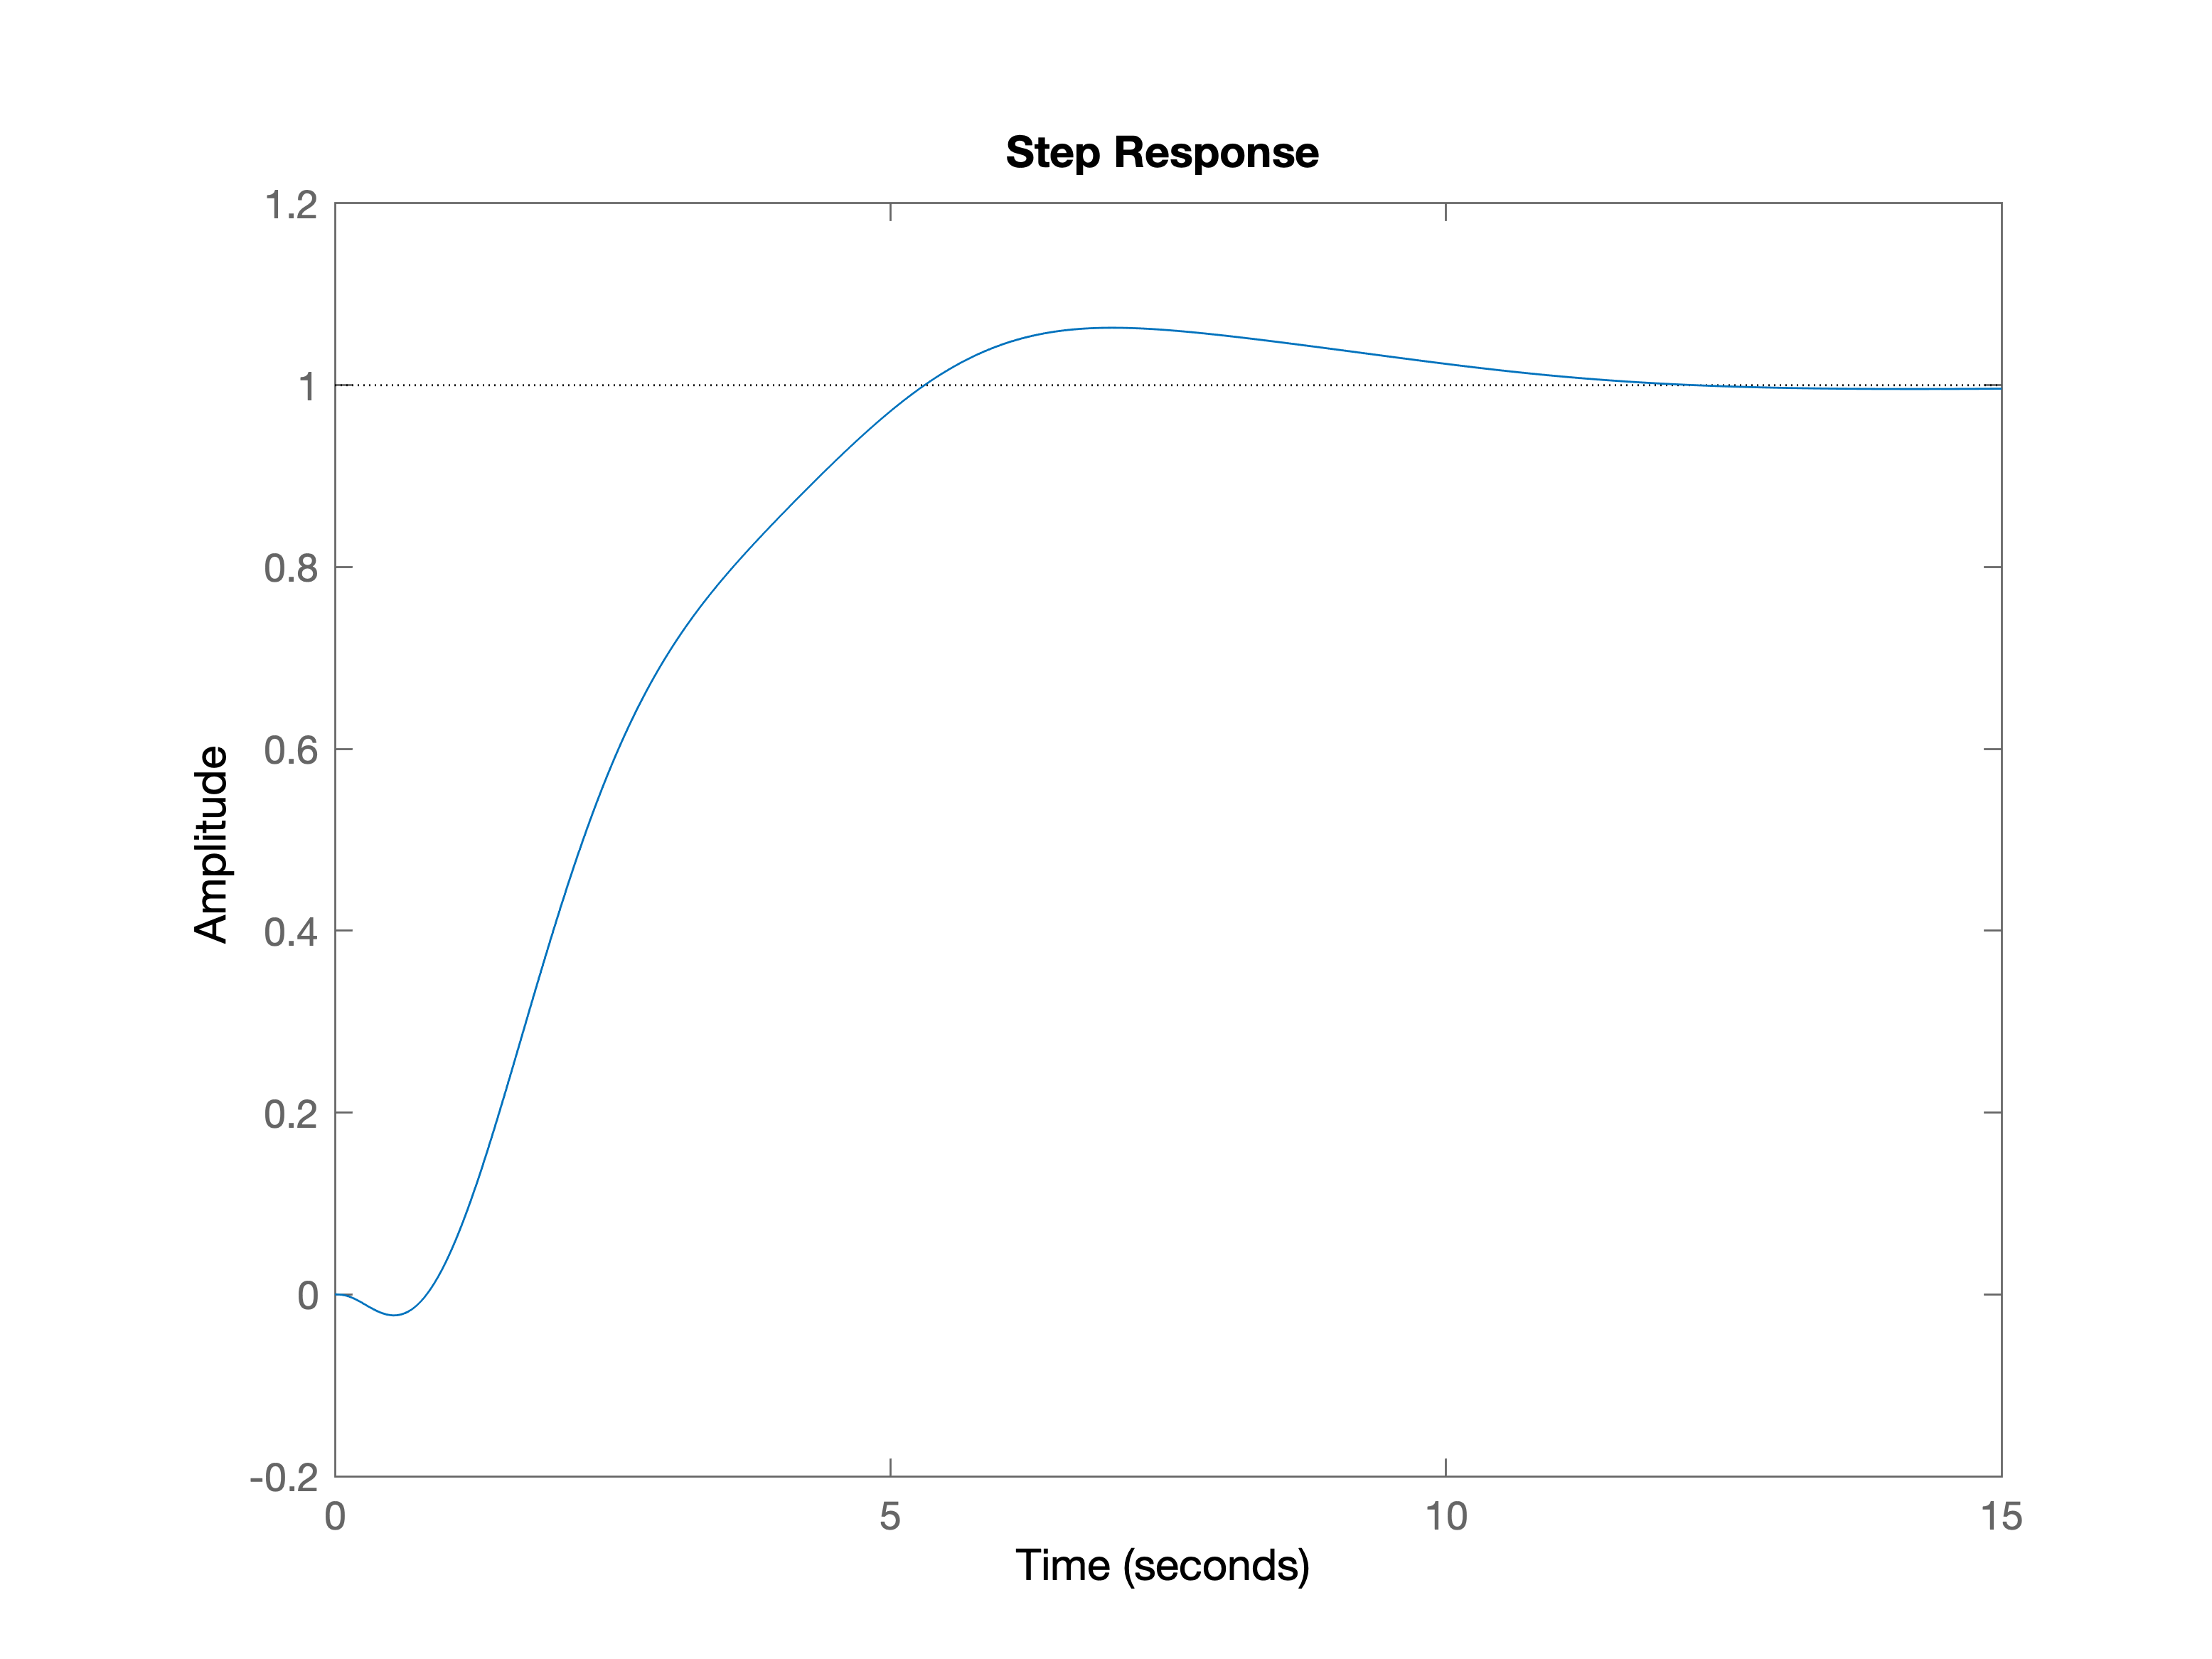
\includegraphics[width=10cm]{../Figure/Q1/b/chr0.png}
    \end{figure}
    \item CHR set point $20\%$ overshoot
    $$
    G_c =   \dfrac{1.758 s^2 + 2.581 s + 1.797}{0.08893 s^2 + 1.371 s}
    $$ 
    \begin{figure}[H]
        \caption{step responde with CHR set point $20\%$ overshoot PID controller}
        \centering
        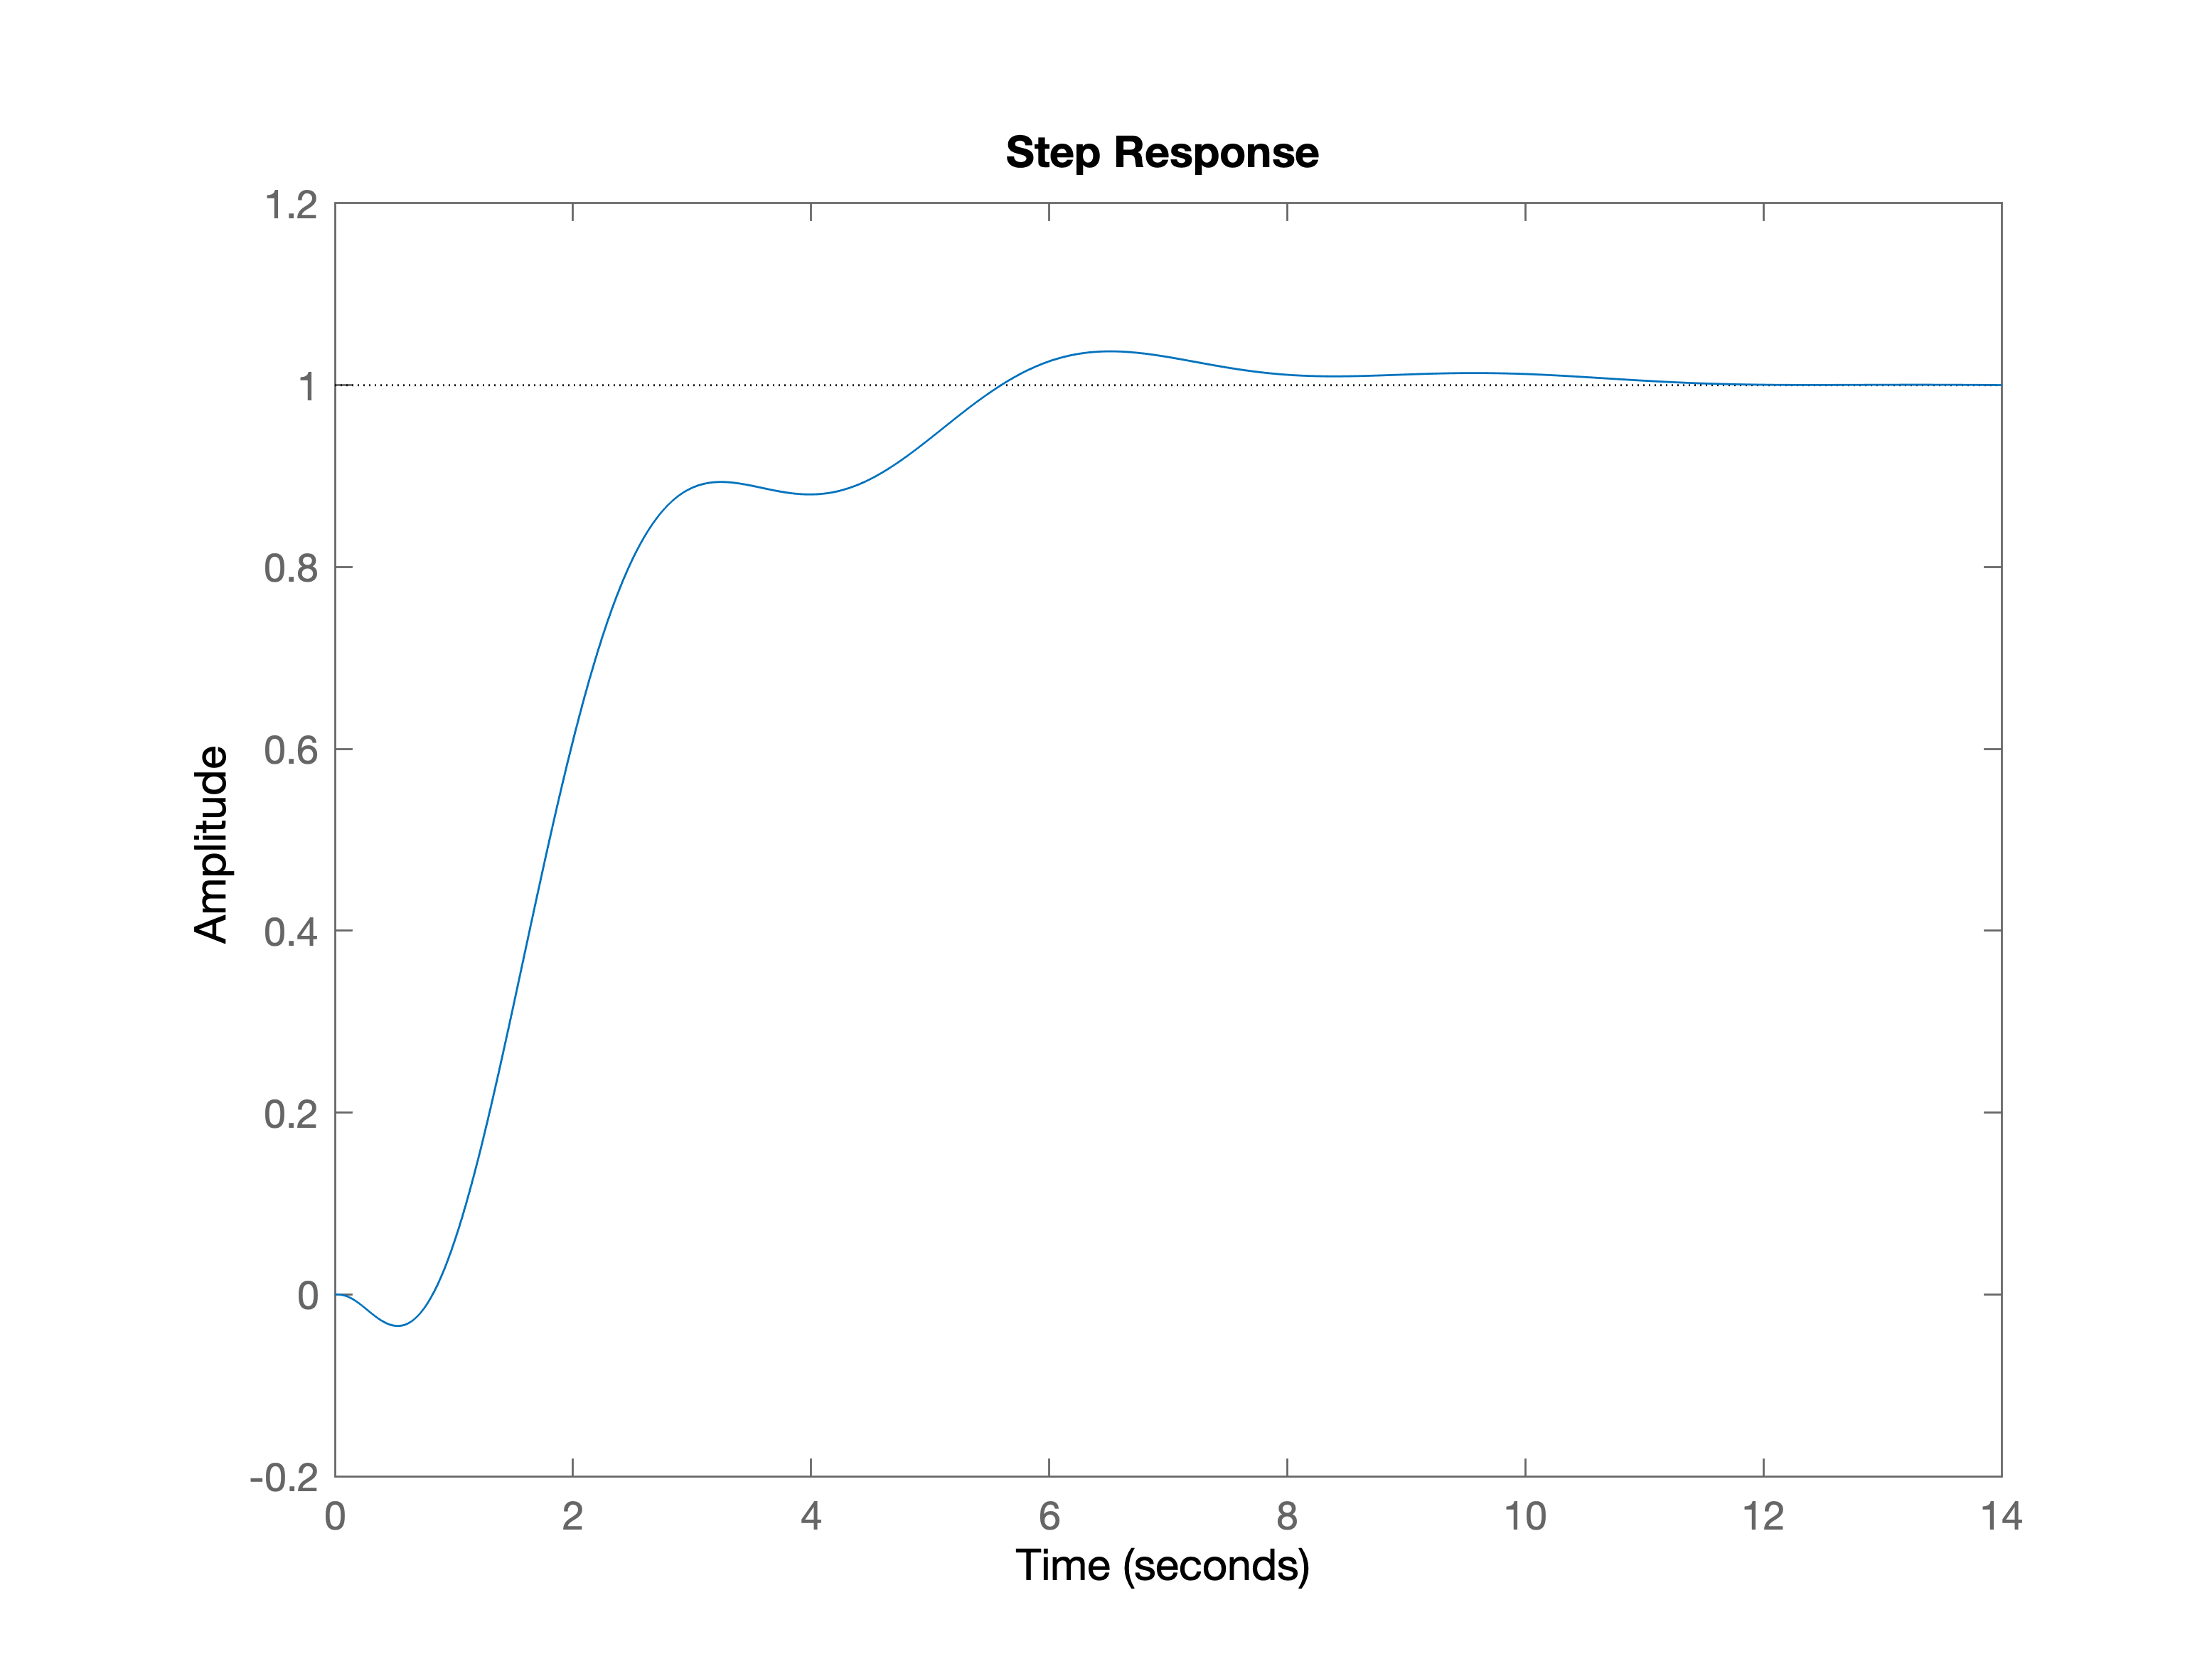
\includegraphics[width=10cm]{../Figure/Q1/b/chr20.png}
    \end{figure}
    \item WJC
    $$
    G_c =   \dfrac{9.298 s^2 + 21.39 s + 12.51}{0.4048 s^2 + 10 s}
    $$ 
    \begin{figure}[H]
        \caption{step responde with WJC PID controller}
        \centering
        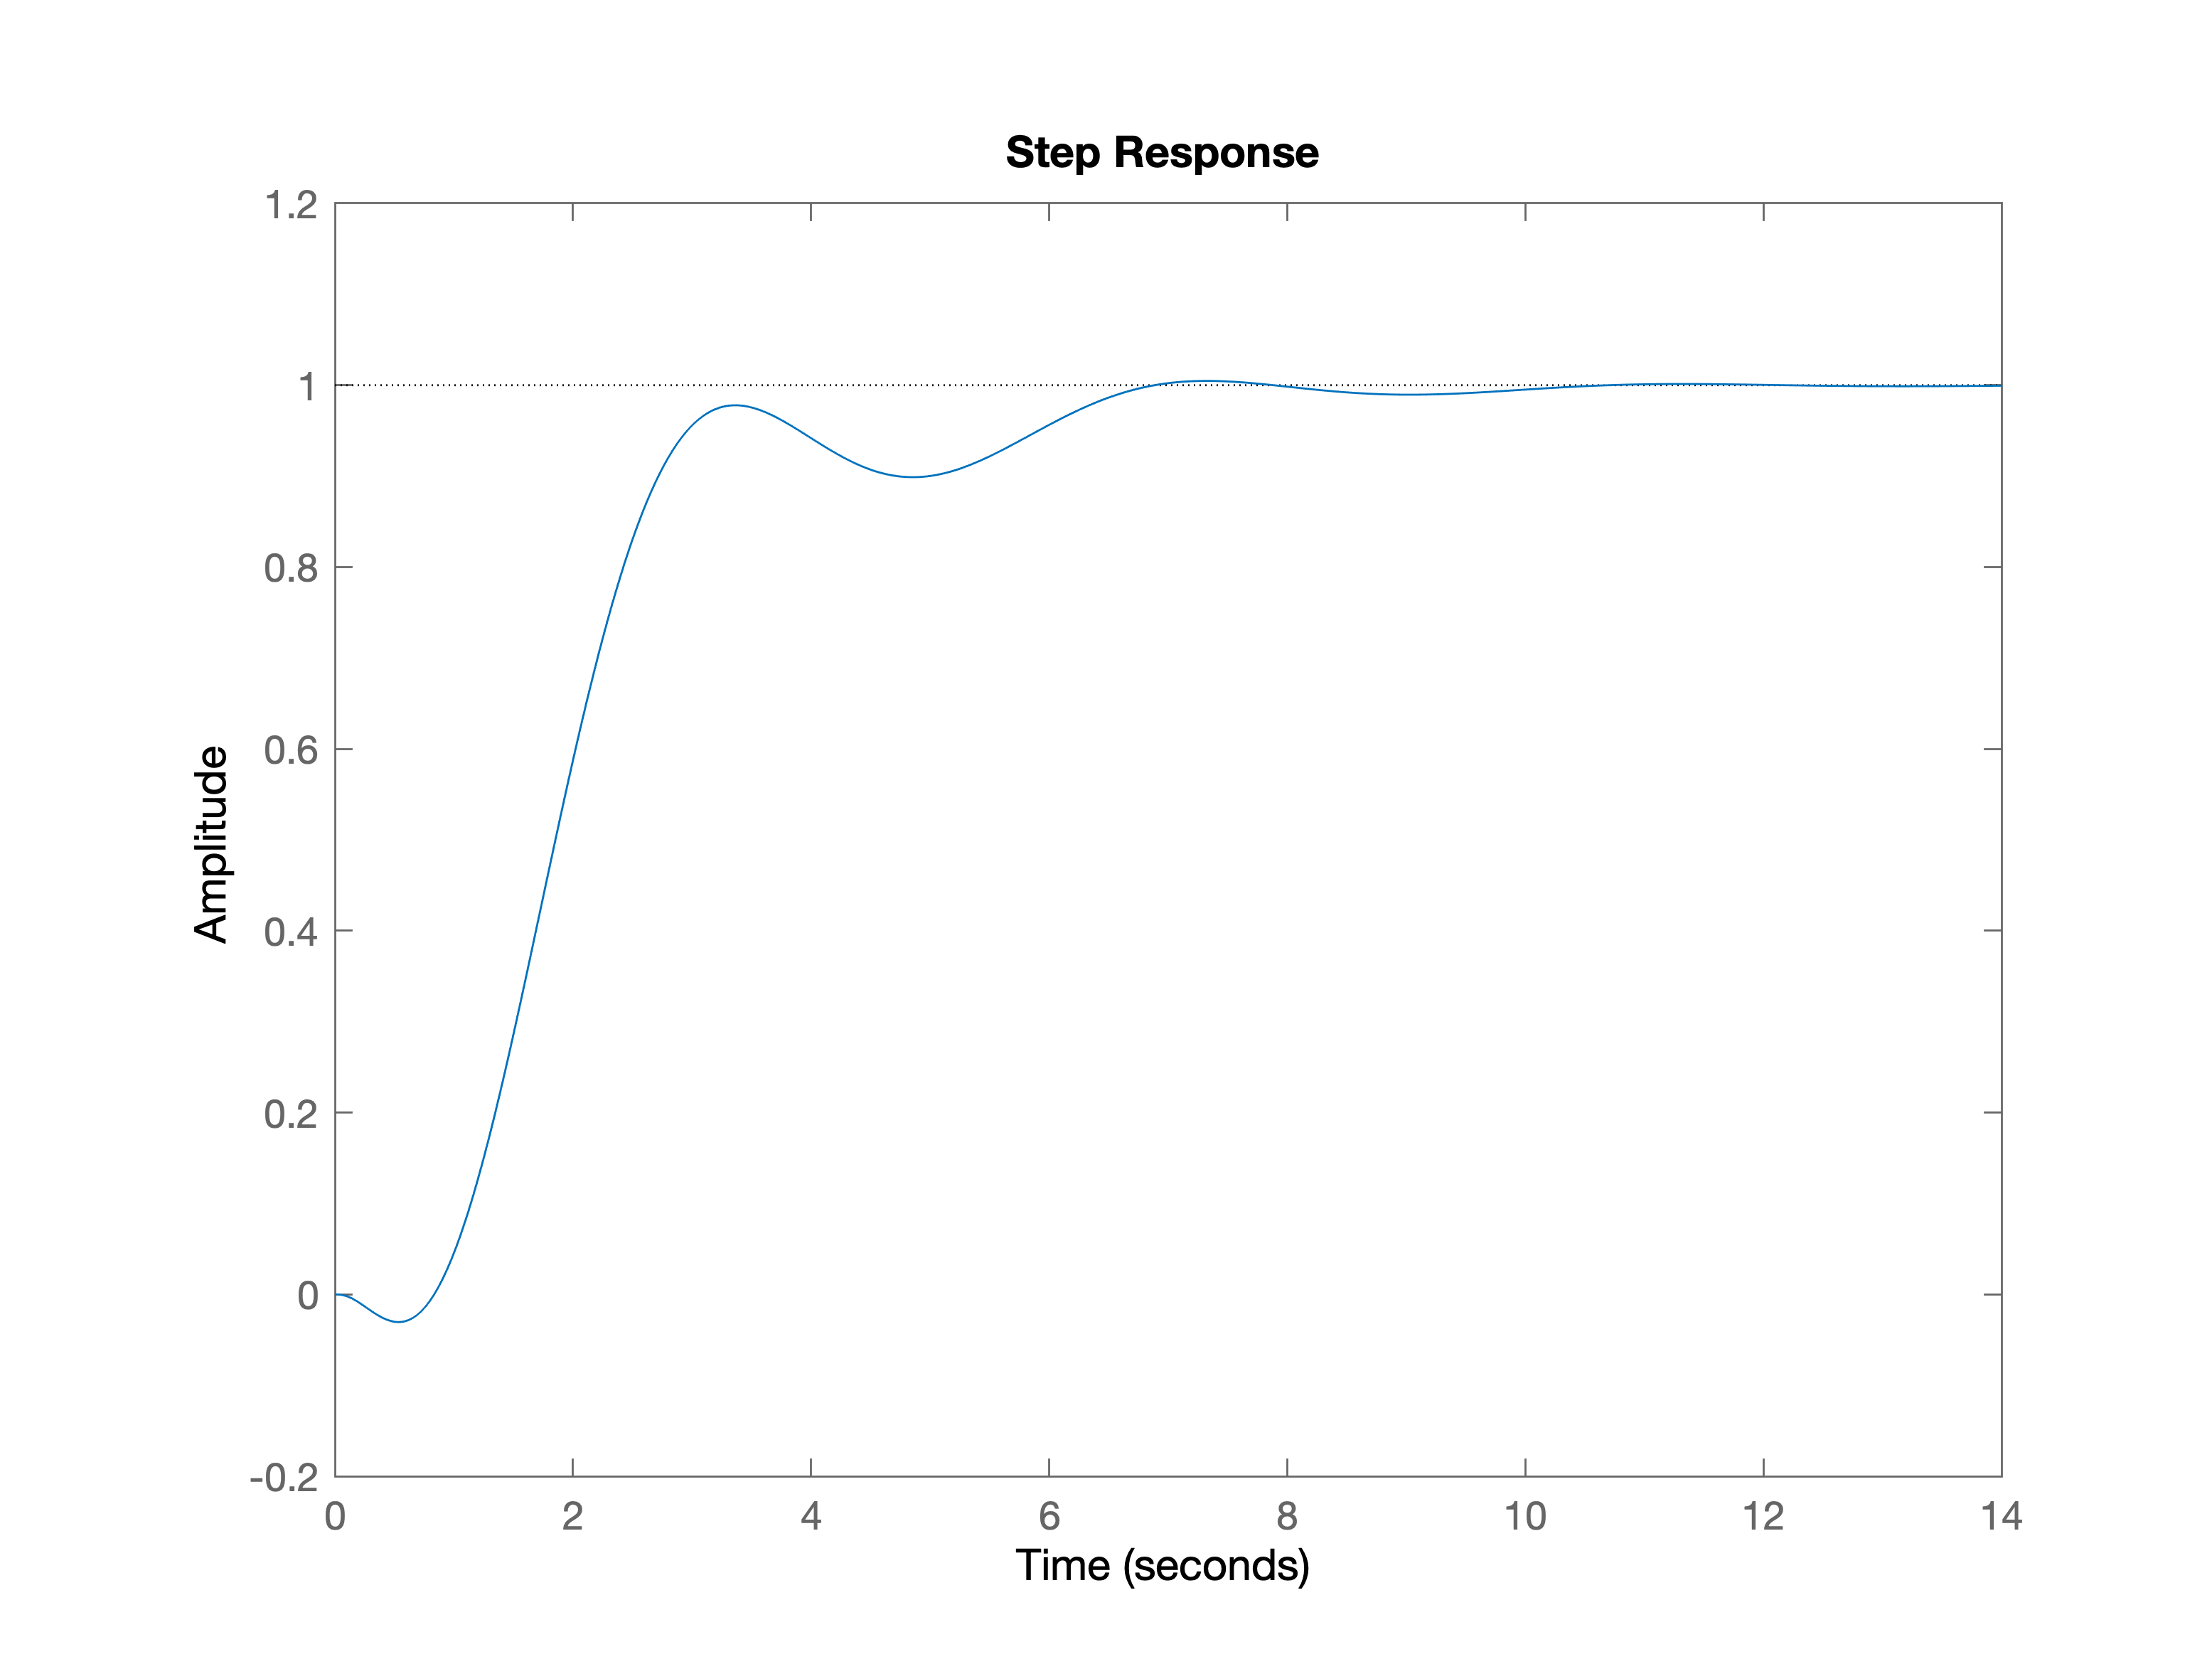
\includegraphics[width=10cm]{../Figure/Q1/b/wjc.png}
    \end{figure}  
    \item optimum set point PID ISTE
    $$
    G_c =   \dfrac{1.993 s^2 + 3.738 s + 2.496}{0.07258 s^2 + 1.447 s}
    $$ 
    \begin{figure}[H]
        \caption{step responde with optimum PID controller}
        \centering
        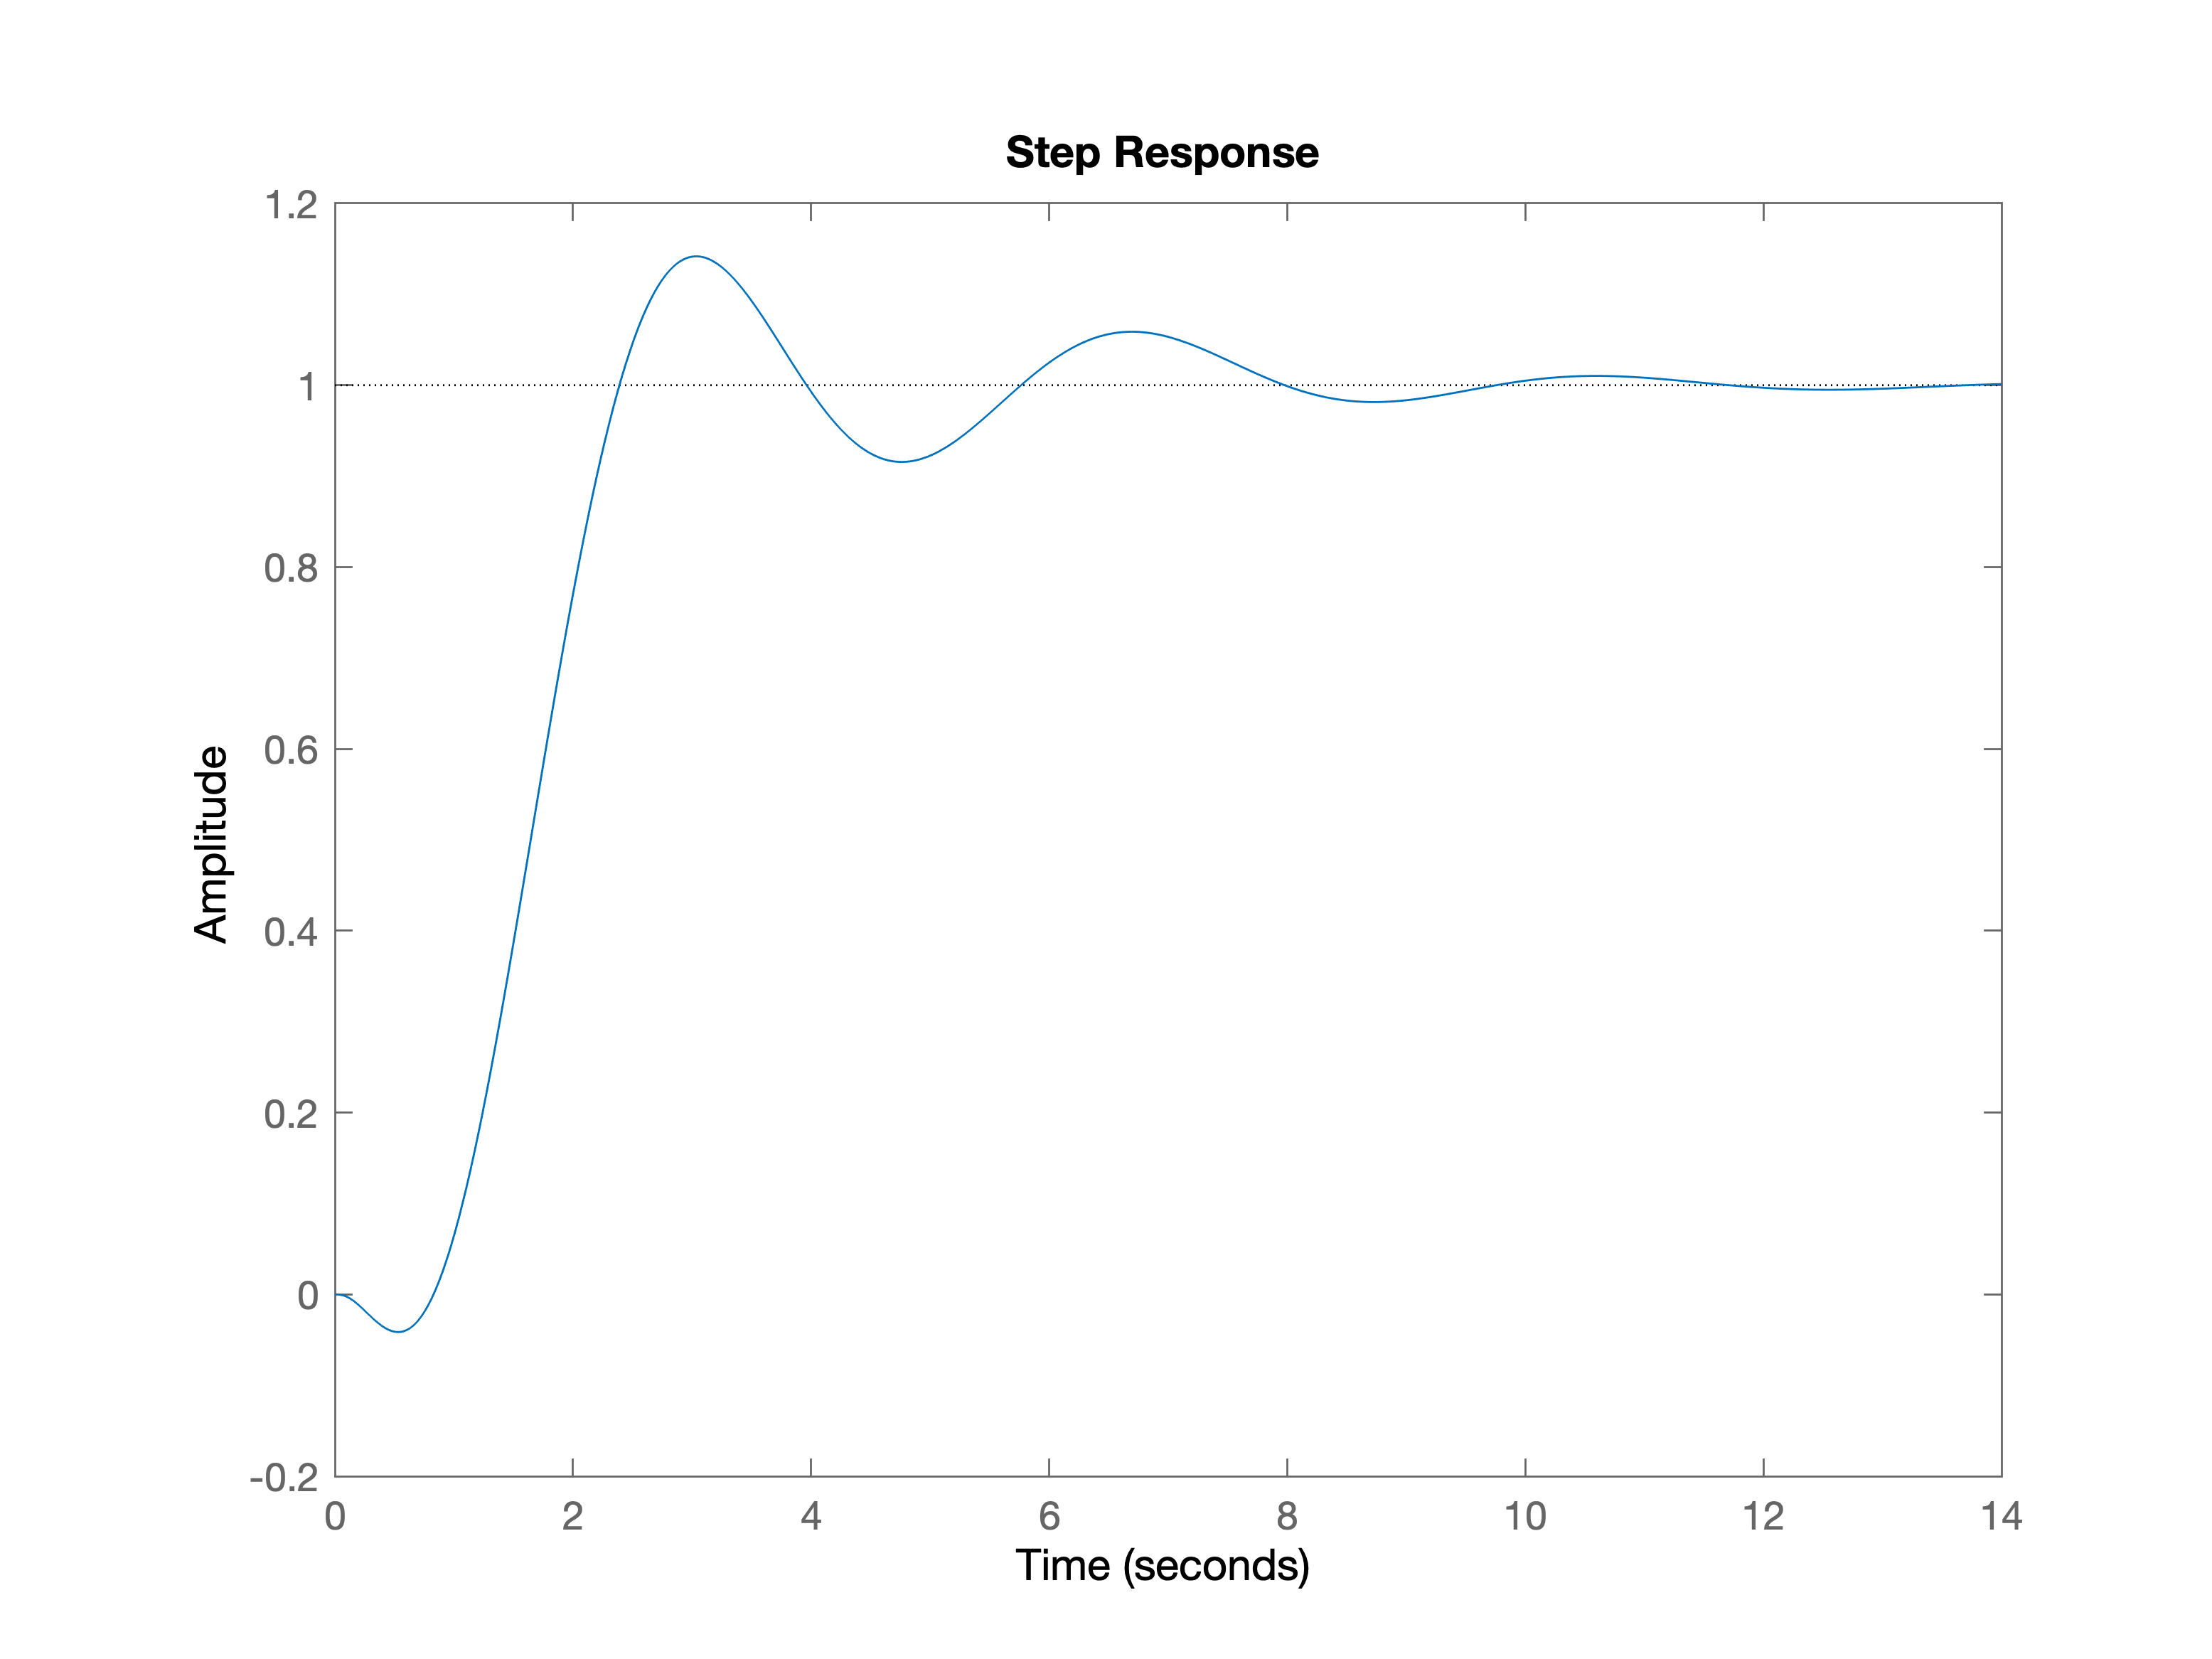
\includegraphics[width=10cm]{../Figure/Q1/b/optpid.png}
    \end{figure}  
    \item optimum set point PI-D ISTE
    $$
    G_c =   \dfrac{4.219 s + 2.41}{1.751 s} \qquad H = \frac{0.9836 s^2 + 4.328 s + 2.41}{0.191 s^2 + 4.328 s + 2.41}
    $$ 
    \begin{figure}[H]
        \caption{step responde with optimum PI-D controller}
        \centering
        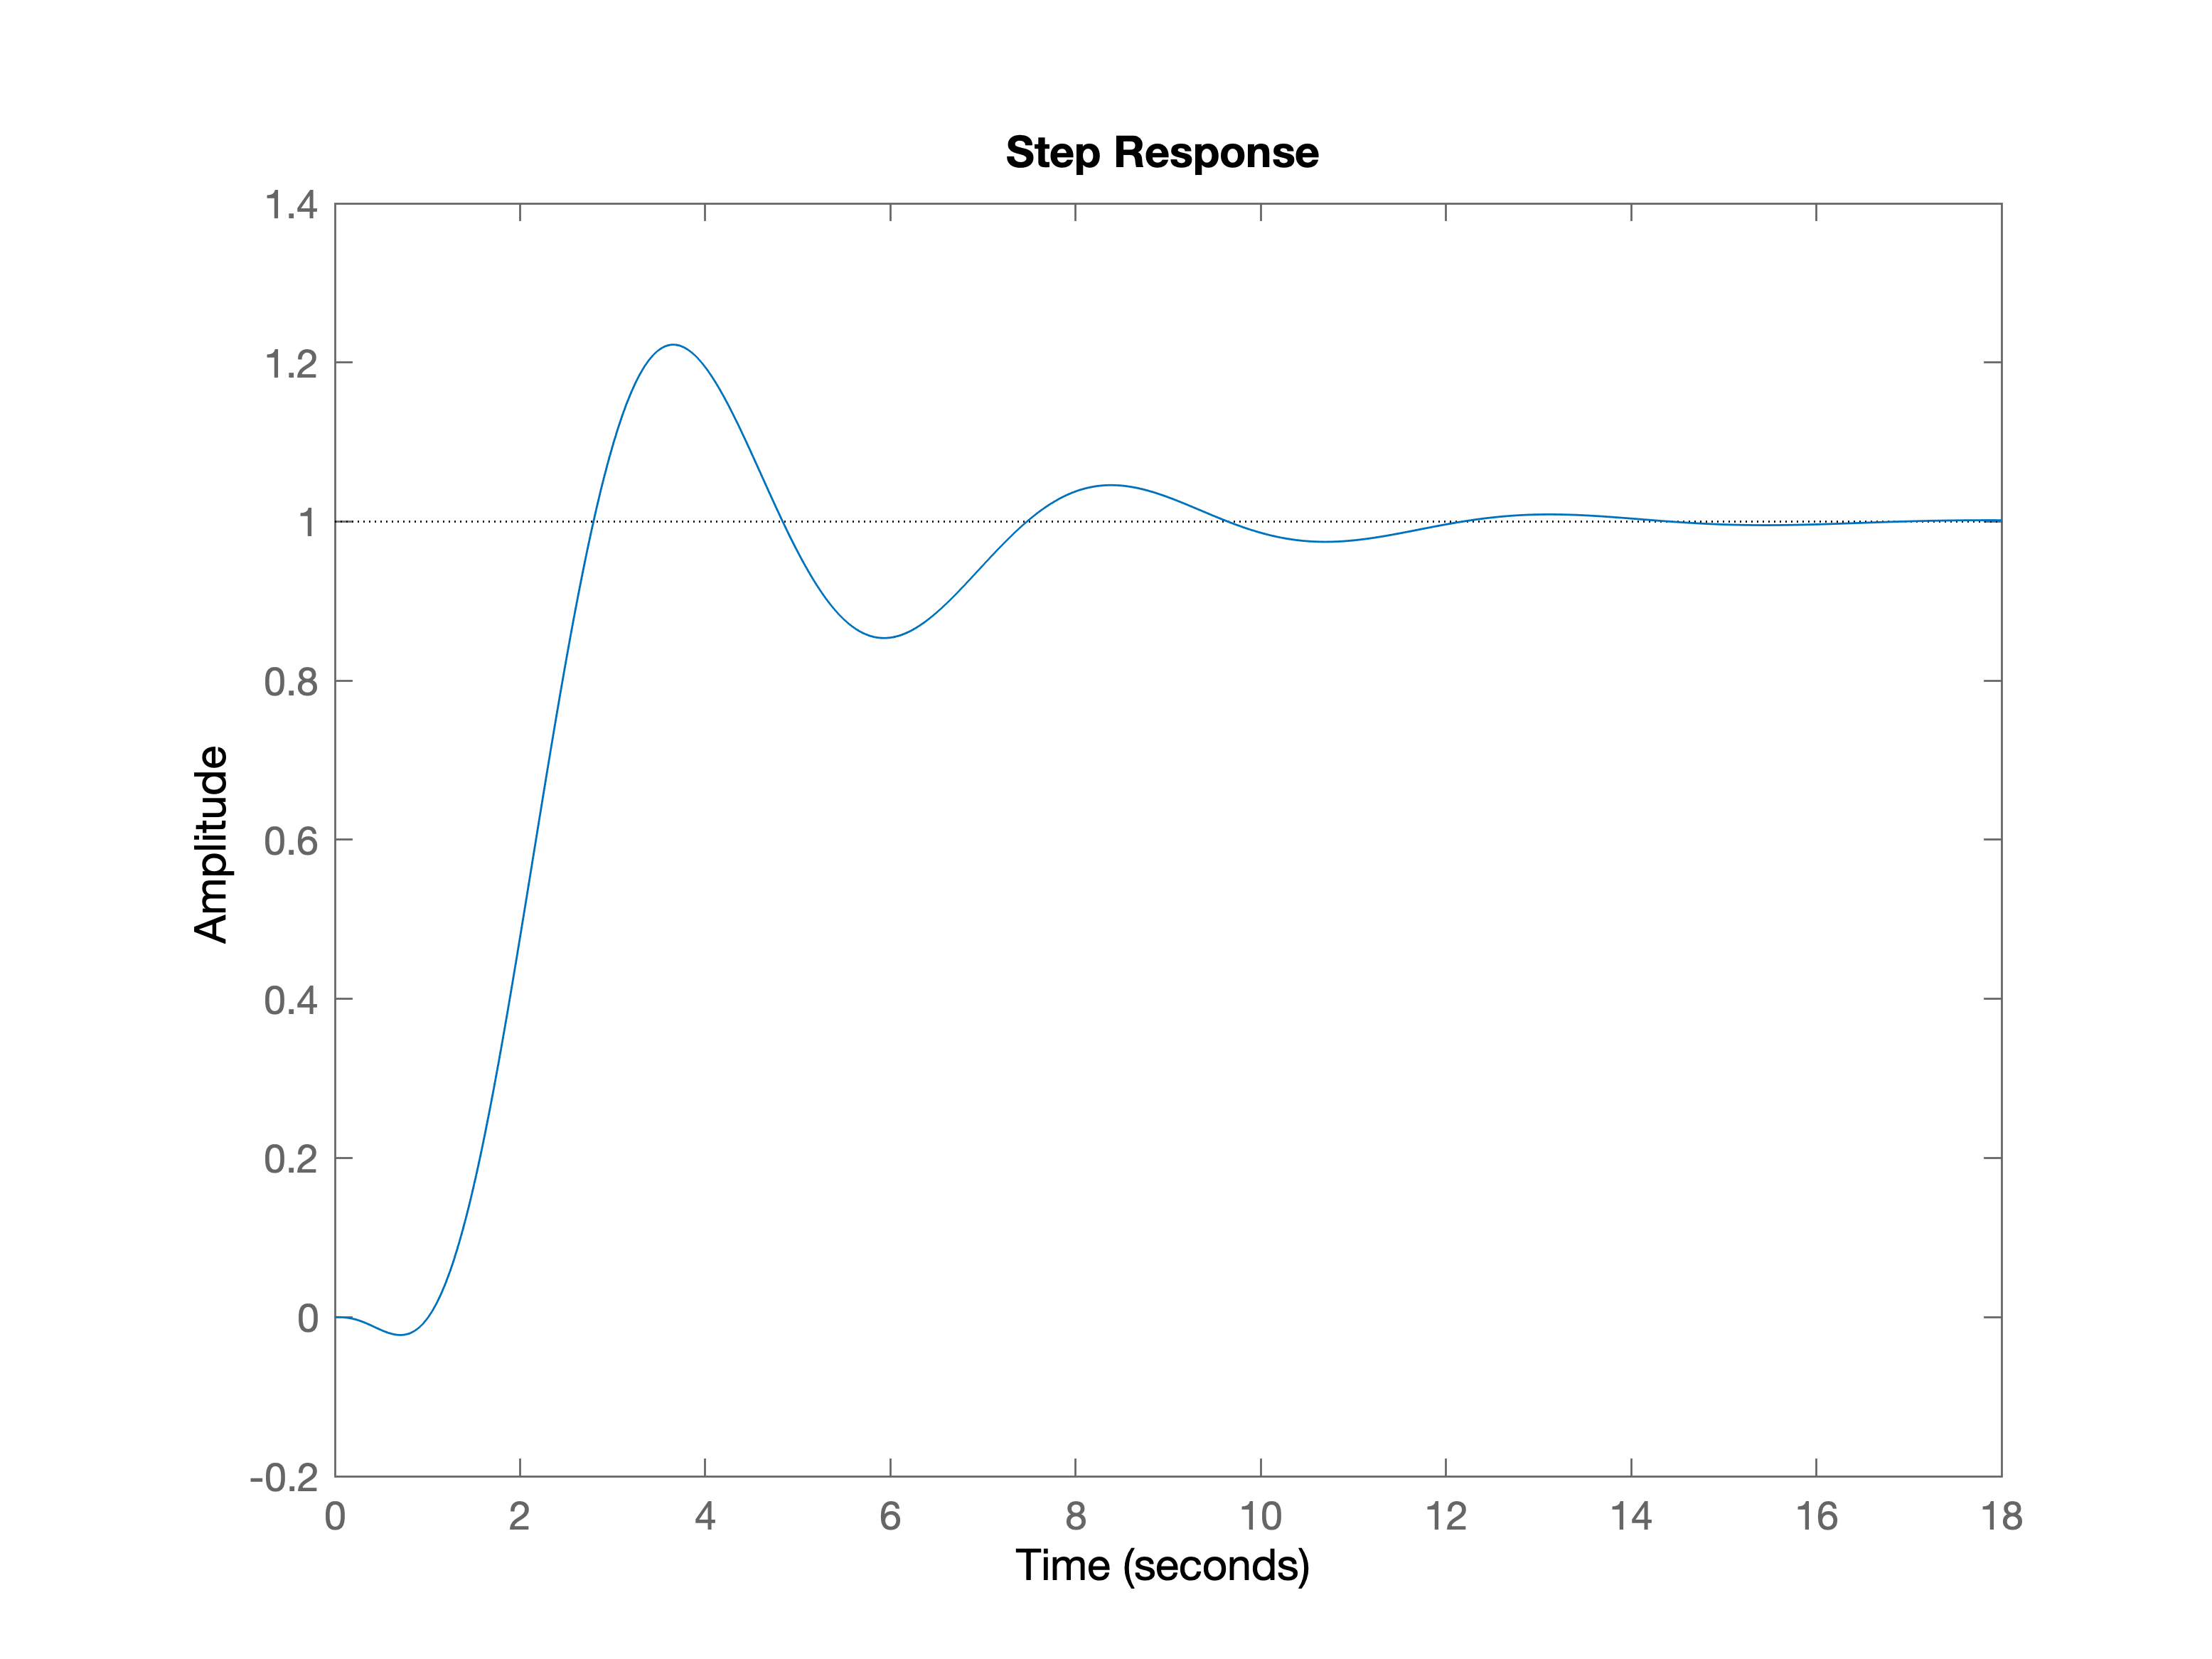
\includegraphics[width=10cm]{../Figure/Q1/b/optpi-d.png}
    \end{figure}  
\end{itemize}
\subsection{conclusion}
ziegler nichols is very slow but refined ziegler nichols is better ans faster. modified ziegler nichols is very slow.
Cohen coon is slow and has hight overshoot but cohen coon revisited is faster.
Astromm hagglund is very good in doesn't have overshoot and system is fast but Frequency is a little slow. CHR is fast but overshoot method work strange. Zero overshoot has overshoot but 20\% overshoot has lower overshoot.
WJC work fast and have very small overshoot.
Optimum PID work well but PI-D is a little slow.
We don't what the system is so we can't select best controller it depends on our plant.
